% main_fr.tex — traduction française fidèle de main.tex, pour relecture interne.
% Ce n'est PAS la version soumise (la soumission APSEC/SEIP se fait en anglais
% depuis main.tex). Mêmes figures, mêmes références, même structure.
\documentclass[10pt,conference]{IEEEtran}
\IEEEoverridecommandlockouts

\usepackage[T1]{fontenc}
\usepackage[utf8]{inputenc}
\usepackage{cite}
\usepackage{amsmath,amssymb,amsfonts}
\usepackage{graphicx}
\usepackage{booktabs}
\usepackage{tabularx}
\usepackage{array}
\usepackage{microtype}
\usepackage{siunitx}
\usepackage{xcolor}
\usepackage{hyperref}
\usepackage{cleveref}
\definecolor{brandgreen}{HTML}{00915A}
\hypersetup{colorlinks=true,allcolors=brandgreen}
\newcommand{\best}[1]{\textbf{#1}}
\newtheorem{proposition}{Proposition}

\newcolumntype{L}[1]{>{\raggedright\arraybackslash}p{#1}}
\newcolumntype{C}[1]{>{\centering\arraybackslash}p{#1}}
\newcommand{\tblsetup}{%
  \footnotesize%
  \setlength{\tabcolsep}{3pt}%
  \renewcommand{\arraystretch}{1.02}%
}

% Espacements de flottants resserrés (budget de pages).
\setlength{\textfloatsep}{7pt plus 2pt minus 3pt}
\setlength{\dbltextfloatsep}{7pt plus 2pt minus 3pt}
\setlength{\floatsep}{7pt plus 2pt minus 2pt}
\setlength{\dblfloatsep}{7pt plus 2pt minus 2pt}
\setlength{\abovecaptionskip}{4pt}

% Francisation des libellés IEEEtran et cleveref.
\renewcommand{\abstractname}{Résumé}
\renewcommand{\IEEEkeywordsname}{Mots-clés}
\renewcommand{\appendixname}{Annexe}
\crefname{figure}{Fig.}{Fig.}
\Crefname{figure}{Fig.}{Fig.}
\crefname{table}{Tab.}{Tab.}
\Crefname{table}{Tab.}{Tab.}
\crefname{section}{Sect.}{Sect.}
\Crefname{section}{Sect.}{Sect.}
\crefname{proposition}{Proposition}{Propositions}
\Crefname{proposition}{Proposition}{Propositions}

\providecommand{\repourl}{https://anonymous.4open.science/r/VERA-A3D7}

\begin{document}

\title{VERA : un framework modulaire orienté AI Act\\ pour l'évaluation de l'IA responsable des LLM}

\author{%
  \IEEEauthorblockN{%
    Robin Qu\'eriaux,
    Mariam Barry,
    L\'ea D\'el\'eris,
    Solveig Bachellery%
  }
  \IEEEauthorblockA{BNP Paribas}%
}

\maketitle

\begin{abstract}
Les organisations qui déploient des grands modèles de langage sous l'EU AI Act sont fortement encouragées à produire des preuves techniques reproductibles sur l'ensemble des principes de l'IA de confiance.
COMPL-AI, un framework introduit en 2024, traduit ces principes en douze exigences mesurables et les rapporte sous la forme d'une étude de benchmarking.
Nous rapportons notre expérience de construction et d'exploitation de VERA (\emph{Verifiable Evaluation for Responsible AI}), un framework open-source d'analyse de risques et d'audit technique des déploiements de LLM qui s'appuie sur COMPL-AI, développé et expérimenté au sein de la fonction IA responsable d'une grande banque européenne.
Quatre capacités opérationnelles répondent à des manques rencontrés en pratique.
VERA génère des artefacts de preuve liés à chaque exécution, susceptibles d'alimenter les analyses de risques et la documentation technique attendues par le règlement.
Il restitue les résultats via un tableau de bord par rôles qu'un non-spécialiste peut piloter sans écrire de code.
Il traite la politique de scoring qui sous-tend chaque score final comme un objet de première classe, signé, et une borne fermée indique quels verdicts sont robustes à une modification des pondérations.
Sa spécification, ses benchmarks et ses poids sont des données interchangeables : VERA exécute COMPL-AI aujourd'hui et peut s'adapter à une autre spécification sans changement de code.
En exploitation, nous avons évalué six LLM à poids ouverts sur des jeux de données publics et un corpus synthétique publié : trois familles de modèles à taille comparable (Llama~3.1~8B, Qwen2.5~7B, Gemma~2~9B), puis trois tailles d'une même famille (Ministral~3B, Mistral~7B, Mistral-Small~24B).
À taille croissante, la capacité, mesure grossière de la performance brute, passe de 0,70 à 3B et 7B à 1,00 à 24B.
Pourtant la résilience cyber chute de 0,50 à 0,00 sur le plus grand modèle, et ce verdict est invariant à toute repondération : un modèle plus grand n'est pas toujours un modèle plus responsable.
Nous partageons les enseignements tirés de la construction et du déploiement du framework.
\end{abstract}

\begin{IEEEkeywords}
Framework, IA responsable, Open source, EU AI Act, COMPL-AI, Benchmark
\end{IEEEkeywords}

\section{Introduction}
\label{sec:introduction}

\begin{figure*}[t]
  \centering
  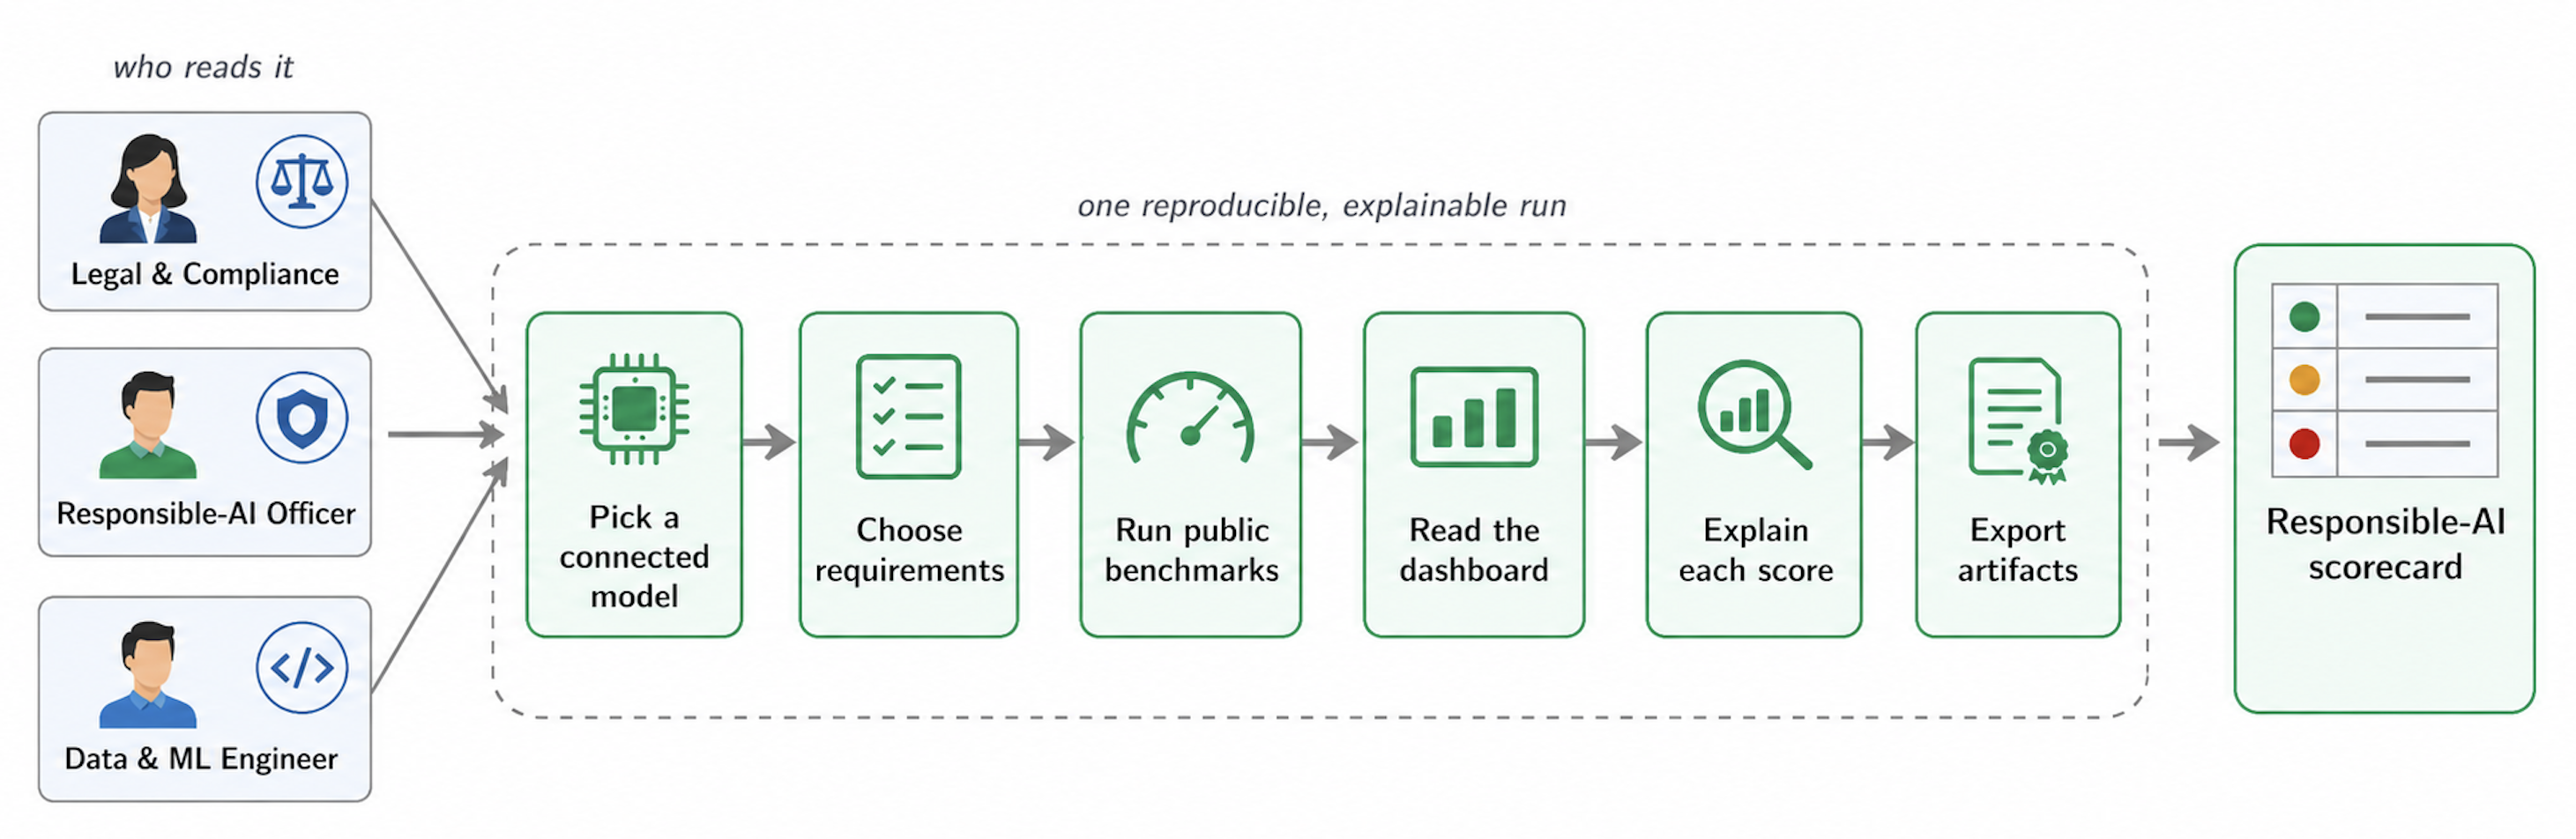
\includegraphics[width=0.80\textwidth]{figures/fig1}
  \caption{Le parcours du framework. Trois rôles pilotent VERA : ils choisissent un modèle connecté, sélectionnent les exigences d'IA responsable à vérifier et exécutent des benchmarks publics ; VERA présente ensuite un tableau de bord par rôles qui explique chaque score avant l'export des artefacts.}
  \label{fig:journey}
\end{figure*}

\subsection{Motivation}
Avant qu'une organisation ne mette en production un assistant fondé sur un LLM dans un cadre réglementé, l'EU AI Act demande des preuves techniques sur l'ensemble de ses principes d'IA de confiance~\cite{euaiact2024}, parmi lesquels la robustesse, la vie privée, la transparence, l'équité et la supervision humaine.
COMPL-AI~\cite{guldimann2024complai}, une opérationnalisation communautaire du règlement, transforme ces principes en douze exigences mesurables.
Il les rapporte sous forme d'une suite de benchmarking open-source, décomposée par principe et par benchmark.
C'est la bonne structure, et nous nous appuyons dessus.
Ce qu'elle laisse au praticien, c'est la dernière étape vers une décision de mise en production.
La suite se pilote en ligne de commande, à destination des ingénieurs ML, et n'est pas conditionnée pour le responsable conformité ou risques qui doit valider.
Son agrégation fige une pondération implicite, une simple moyenne, et ne quantifie pas comment ce choix façonne un verdict.
Elle ne dit pas à quelle distance de l'échec se situe une exigence qui passe, ni quels verdicts basculeraient sous une pondération différente et tout aussi défendable.
Une décision de mise en production ne gagne pas grand-chose à un nombre de plus.
Elle appelle une vue par critère dont la politique de scoring est explicite et auditable, et un énoncé de ceux des verdicts qui y sont robustes.
VERA est né de ce besoin précis au sein de la fonction IA responsable d'une grande banque européenne, où les décisions de mise en production d'assistants fondés sur des LLM relèvent des responsables conformité et risques, sous obligations de contrôle interne ; il a été construit dans le cadre d'une collaboration industrie-académie et est publié en open source.

\subsection{Contributions}
Nous présentons VERA, un framework open-source qui exécute les douze exigences mesurables de COMPL-AI, rend signée et auditable la politique d'agrégation derrière chaque score, et quantifie la robustesse de chaque verdict à cette politique.
Les six exigences non mesurables suivent un chemin humain traçable dans le même outil : une file de revue fondée sur une grille de critères, un rapport énergétique mesuré et des formulaires déclaratifs signés.
Les scores restent explicables au sens décompositionnel : chaque score d'exigence est traçable, à l'intérieur de l'outil, jusqu'aux benchmarks publics contributeurs et à leurs résultats individuels.
VERA offre quatre capacités opérationnelles, chacune répondant à un manque rencontré en pratique, chacune associée à une question de recherche, et chacune constituant un écart concret vis-à-vis des deux travaux les plus proches : l'implémentation de référence de COMPL-AI et PromptOps~\cite{sunetnanta2025promptops}.
\begin{itemize}
  \item \textbf{C1 (tableau de bord opérable).} VERA restitue les métriques mesurables de COMPL-AI\footnote{Projet COMPL-AI : \url{https://compl-ai.org}.} via un tableau de bord par rôles qu'un non-spécialiste peut piloter de bout en bout, lancer une exécution et lire ses verdicts, sans écrire de code (RQ1). Nous étayons cette affirmation par une petite étude utilisateur auto-administrée ($n{=}5$) en \Cref{sec:results}. COMPL-AI livre une étude en ligne de commande et un classement public par principe destinés aux ingénieurs ML ; PromptOps rapporte des tableaux de scores plats. L'écart porte sur l'opérabilité pour un non-spécialiste, pas sur la visualisation en tant que telle.
  \item \textbf{C2 (traçabilité liée à l'exécution).} Nous lions les artefacts de preuve à l'évaluation qui les a produits : chaque exécution génère sa propre model card et, pour les exécutions sur jeu de données, une datasheet, renseignées à partir de cette évaluation précise ; COMPL-AI n'émet pas de tels artefacts liés à l'exécution. Ces artefacts peuvent alimenter l'analyse de risques d'un fournisseur et sa documentation technique au titre de l'annexe~IV ; ils ne constituent ni ne remplacent l'une ou l'autre. Dans le tableau de bord, chaque verdict se décompose également en ses benchmarks contributeurs, de sorte qu'un non-spécialiste voit \emph{pourquoi} une exigence est faible (RQ2). La décomposition elle-même suit le reporting hiérarchique de COMPL-AI ; l'apport de recherche est de lier décomposition, exécution et documentation signée en un seul objet auditable.
Le même chemin lié à l'exécution couvre les six exigences non mesurables : chaque exécution met automatiquement en file une revue humaine sur grille pour l'explicabilité (N01) et la corrigibilité (N02), mesure l'énergie pour N03, et atteste N04 à N06 via des formulaires déclaratifs signés.
  \item \textbf{C3 (scoring auditable et interchangeable).} La politique de scoring est un catalogue versionné et signé dont l'empreinte SHA-256 est épinglée dans chaque exécution, et une borne fermée (\Cref{prop:range}) quantifie la dépendance de chaque verdict à cette politique (RQ4), là où COMPL-AI fixe une moyenne non pondérée et laisse cette dépendance non mesurée. La spécification des exigences, les benchmarks et les poids sont eux-mêmes des données interchangeables, et nous l'avons éprouvé : une spécification alternative orientée sécurité est livrée sous forme de deux fichiers de données et s'est exécutée de bout en bout par simple configuration (RQ3). C'est pourquoi nous parlons d'un framework.
  \item \textbf{C4 (étude reproductible).} Nous rapportons une étude ouverte et reproductible des douze exigences sur deux panels de modèles, trois familles à taille comparable et une famille sur trois tailles, avec des jeux de données publics et un corpus synthétique publié. La valeur réside dans le protocole signé et reproductible à travers familles et tailles, appliqué aux modèles que nous évaluons réellement en pratique ; les résultats inter-modèles sont des constats.
\end{itemize}
Nous évaluons C1--C4 sur les deux panels de \Cref{sec:results}, où VERA signale des écarts concrets d'IA responsable entre familles et entre tailles.

\smallskip\noindent\textbf{Disponibilité et reproductibilité.}
VERA est open-source et disponible à l'adresse \url{\repourl}. Le paquet de réplication publié (graine~42) régénère chaque tableau et chaque figure de cet article, y compris le catalogue signé et l'étude de sensibilité des verdicts.

\section{Contexte et travaux connexes}
\label{sec:related}

\subsection{Cadre réglementaire et COMPL-AI}
L'EU AI Act~\cite{euaiact2024} suit une approche par les risques.
Il interdit un ensemble restreint de pratiques ; il impose gestion des risques, documentation technique et supervision humaine aux systèmes à haut risque listés à son annexe~III ; il fixe des obligations de transparence pour les usages à risque limité tels que les assistants IA (art.~50) ; et il laisse les systèmes à risque minimal largement libres.
Des preuves techniques sont demandées aux systèmes à haut risque, et les principes éthiques derrière ces obligations s'inspirent des lignes directrices non contraignantes du HLEG~\cite{hleg2019trustworthyai}.
Les cadres du NIST et de l'ISO~\cite{nist2023airmf,iso42001_2023} guident la gestion des risques organisationnels, mais s'arrêtent avant les métriques exécutables.
Des travaux antérieurs en génie logiciel extraient et vérifient des exigences réglementaires avec des techniques de TAL et de LLM, y compris sur l'AI Act lui-même~\cite{abualhaija2025llmregextraction,amaral2022nlpcompliance,abualhaija2024regchange}.
VERA est complémentaire : il n'analyse pas le texte réglementaire mais opérationnalise une taxonomie d'exigences existante en une évaluation exécutable et auditable.
COMPL-AI~\cite{guldimann2024complai} réduit l'écart sur les métriques.
Il s'agit d'un effort indépendant d'ETH Zurich, de l'INSAIT et de LatticeFlow AI : il n'est pas financé par l'UE, ne fait pas partie des normes harmonisées du règlement, et un porte-parole de la Commission européenne l'a décrit comme une première étape vers l'opérationnalisation du règlement.
Il regroupe les principes éthiques du règlement en six domaines et les associe à dix-huit exigences techniques, dont douze avec des scores mesurables dans $[0,1]$.
Il livre également sa propre suite d'évaluation open-source (27 benchmarks) et un classement public.
Les six exigences restantes demeurent non évaluées dans son étude : les auteurs notent que des outils de mesure adéquats n'existent pas encore, et les rapportent comme N/A ou comme constantes triviales.
Nous énonçons clairement le recouvrement : VERA implémente la taxonomie mesurable de COMPL-AI et exécute la même famille de benchmarks publics.
COMPL-AI rapporte déjà ses résultats de façon décompositionnelle, sous forme d'une hiérarchie principe, exigence, benchmark, avec des journaux au niveau des échantillons et une vue publique par principe, et il est extensible par la communauté ; VERA ne revendique comme nouveauté ni la décomposition ni l'extensibilité.
Les apports de VERA sont quatre propriétés que COMPL-AI n'offre pas.
Premièrement, une politique de scoring signée et épinglée par empreinte, assortie d'une analyse fermée de sensibilité des verdicts : COMPL-AI agrège chaque exigence par une moyenne non pondérée et ne quantifie pas comment ce choix façonne un verdict.
Deuxièmement, des model cards et des datasheets liées à l'exécution.
Troisièmement, une interface opérable et par rôles pour les non-spécialistes, avec un mode optionnel de gouvernance à l'exécution.
Quatrièmement, un chemin humain traçable pour les six exigences non mesurables, une file de revue sur grille assortie de formulaires d'attestation signés, là où COMPL-AI s'arrête à N/A.

\subsection{Suites de benchmarks et métriques}
VERA réutilise des suites publiques établies plutôt que de proposer une nouvelle science du benchmark.
La capacité (CR06) s'appuie sur MMLU~\cite{hendrycks2021mmlu}, GSM8K~\cite{cobbe2021gsm8k}, HumanEval~\cite{chen2021humaneval}, TruthfulQA~\cite{lin2022truthfulqa} et BBH~\cite{suzgun2023bbh}.
La calibration (CR07) utilise l'erreur de calibration attendue~\cite{guo2017calibration}.
L'équité et les biais (CR10--CR11) utilisent BBQ~\cite{parrish2022bbq}, BOLD~\cite{dhamala2021bold}, StereoSet~\cite{nadeem2021stereoset} et des métriques de disparité~\cite{hardt2016equality,wang2023decodingtrust}.
La toxicité (CR12) utilise RealToxicityPrompts~\cite{gehman2020realtoxicity}.
Les contrôles au stade des données (CR03--CR05) appliquent des heuristiques de corpus ; les attaques par appartenance et par extraction~\cite{carlini2021membership,carlini2023extracting} motivent des contrôles simplifiés.
Le tatouage numérique (CR09) suit une heuristique statistique inspirée de~\cite{kirchenbauer2023watermark}, et non SynthID en production.
Chaque suite répond à une question de mesure isolément.
Aucune ne les conditionne pour un non-spécialiste ni n'explique un verdict, ce que VERA ajoute.

\subsection{Documentation à l'appui de l'analyse de risques}
L'EU AI Act attend une documentation technique pour les systèmes à haut risque, dont le contenu est fixé par la loi (art.~11, annexe~IV).
La communauté réutilise deux formats : les Model Cards~\cite{mitchell2019modelcard} et les Datasheets for Datasets~\cite{gebru2021datasheets}.
Ces documents sont souvent produits après l'exécution, ce qui peut les laisser dériver de l'évaluation qu'ils décrivent.
VERA génère au contraire une model card, et une datasheet pour les exécutions sur jeu de données, directement à partir de chaque évaluation.
L'artefact reste donc lié à l'exécution exacte qui l'a produit ; c'est une preuve d'appui qui peut alimenter la documentation de l'annexe~IV, non un substitut à celle-ci.

\subsection{Frameworks open-source d'évaluation de LLM}
Plusieurs frameworks open-source évaluent les LLM, chacun à un niveau différent.
HELM~\cite{liang2023helm} standardise les scénarios à rapporter.
La suite lm-evaluation~\cite{gao2021lmevalharness} standardise la manière d'exécuter un benchmark.
Garak~\cite{derczynski2024garak} sonde les contournements et les injections de prompt, et DecodingTrust~\cite{wang2023decodingtrust} est une suite de confiance.
Ce sont de solides briques de mesure, et VERA les réutilise plutôt que de les concurrencer.
Ce qu'elles laissent de côté, c'est une vue explicable au niveau des exigences pour un non-spécialiste, et une manière modulaire de changer la spécification sous-jacente.
VERA fournit cette couche au-dessus de la taxonomie COMPL-AI.

\subsection{Articles d'outils en génie logiciel}
Le \Cref{tab:related-work} positionne VERA face aux outils voisins.
PromptOps~\cite{sunetnanta2025promptops} est l'un des outils récents de confiance pour les LLM.
Il note un modèle prompt par prompt et rapporte un ensemble plat de nombres, sans couverture du stade des données, sans explication par critère, ni taxonomie modulaire.
VERA diffère sur trois axes : il associe les résultats à la taxonomie complète CR01--CR12 de COMPL-AI, il explique chaque verdict en le décomposant entre critères et benchmarks publics, et son registre ainsi que sa taxonomie sont enfichables, de sorte que le framework s'adapte au-delà de COMPL-AI.
Les structures explicites de questions de recherche~\cite{liu2022mscpdp} et la conception d'expériences contrôlées~\cite{weninger2018usecase} informent l'organisation de notre évaluation.

\begin{table*}[t]
  \caption{Outils open-source d'évaluation de LLM selon les propriétés visées par VERA. Les cellules indiquent Oui, Partiel, Limité ou Non ; lorsque c'est plus précis, elles nomment la couverture exacte (identifiants d'exigences, Définition) ou la surface offerte (Classement).}
  \label{tab:related-work}
  \centering
  \tblsetup
  \begin{tabularx}{\textwidth}{@{}l*{7}{>{\centering\arraybackslash}X}@{}}
    \toprule
    Outil / framework & Couverture COMPL-AI & Pipeline automatisé & Scoring explicable & Sensibilité du verdict & Tableau de bord & Modulaire / extensible & Auto-hébergé \\
    \midrule
    COMPL-AI~\cite{guldimann2024complai} & Définition & Oui & Partiel & Non & Classement & Partiel & Oui \\
    HELM~\cite{liang2023helm} & Non & Oui & Partiel & Non & Classement & Partiel & Oui \\
    lm-evaluation~\cite{gao2021lmevalharness} & Non & Oui & Non & Non & Non & Oui & Oui \\
    Garak~\cite{derczynski2024garak} & CR02 & Oui & Non & Non & Non & Oui & Oui \\
    DecodingTrust~\cite{wang2023decodingtrust} & Partiel & Partiel & Partiel & Non & Non & Non & Oui \\
    PromptOps~\cite{sunetnanta2025promptops} & Partiel & Oui & Limité & Non & Limité & Non & Oui \\
    \best{VERA (le nôtre)} & \best{CR01--12} & \best{Oui} & \best{Oui} & \best{Oui} & \best{Oui} & \best{Oui} & \best{Oui} \\
    \bottomrule
  \end{tabularx}
  \footnotesize\par\smallskip
  Scoring explicable : \emph{Oui} = chaque verdict d'exigence se décompose, dans l'outil, en ses benchmarks contributeurs et leurs résultats respectifs ; \emph{Partiel} = les résultats par benchmark sont publiés mais non reliés aux verdicts d'exigences dans un outil opérable ; \emph{Limité} = scores plats par test uniquement.
  Sensibilité du verdict : l'outil quantifie-t-il la dépendance de chaque verdict à la pondération d'agrégation (\Cref{sec:rq4}).
\end{table*}

\section{Framework VERA et architecture}
\label{sec:framework}

\subsection{Vue d'ensemble conceptuelle}
VERA transforme un modèle et un ensemble choisi d'exigences d'IA responsable en une fiche de score explicable que différents rôles peuvent lire.
La \Cref{fig:journey} montre le parcours.
Un utilisateur choisit un modèle connecté, sélectionne les exigences à vérifier et lance une exécution.
VERA évalue alors chaque exigence à l'aide de benchmarks publics, agrège les résultats en un score par critère, et les présente dans un tableau de bord par rôles qui explique chaque verdict.

L'idée fondatrice est qu'un unique score global de conformité est sémantiquement pauvre, voire dangereux.
Il masque pourquoi un modèle échoue, et il crée des falaises réglementaires où un petit changement fait basculer un succès en échec.
De plus, l'IA responsable ne signifie pas la même chose pour chaque acteur.
VERA remplace donc le nombre unique par une vue par critère et des tableaux de bord ségrégés par rôle (\Cref{sec:dashboard}) pour trois profils : un responsable juridique ou conformité, un responsable IA responsable, et un ingénieur data ou ML.
Concrètement, une cible peut être un point de terminaison de modèle, un point de contrôle d'entraînement ou un jeu de données, étiqueté par un stade du cycle de vie dans un fichier d'exécution déclaratif.
La section suivante détaille le moteur qui l'exécute (\Cref{fig:architecture}).

\subsection{Architecture du système}
La \Cref{fig:architecture} montre comment VERA transforme une demande de lancement en une exécution scorée et documentée.
Un utilisateur entre par l'une des trois surfaces : la ligne de commande \texttt{vera-eval}, le point de terminaison REST \texttt{POST /runs}, ou l'assistant guidé sans authentification.
Les trois placent la même tâche déclarative dans une file de tâches en arrière-plan (Celery et Redis), qui héberge aussi le magasin d'exécutions et le coupe-circuit.
Un worker exécute ensuite un contrôleur en deux étapes (LangGraph) : une étape \texttt{evaluate} et une étape \texttt{aggregate}.
L'étape \texttt{evaluate} résout chaque exigence en ses benchmarks via un registre, distribue chacun à son exécuteur, et route l'inférence à travers un routeur de modèles auto-hébergé (LiteLLM) vers la cible et un juge.
L'étape \texttt{aggregate} combine les scores par item mis en cache en un score par exigence, avec des intervalles bootstrap, en utilisant le catalogue de benchmarks modulaire.
L'exécution émet ses artefacts, le fichier d'exécution, une model card, les sorties par item et une signature de contenu, vers un stockage objet ou le système de fichiers local, et une API de lecture les sert au tableau de bord (\Cref{sec:dashboard}).

\begin{figure*}[t]
  \centering
  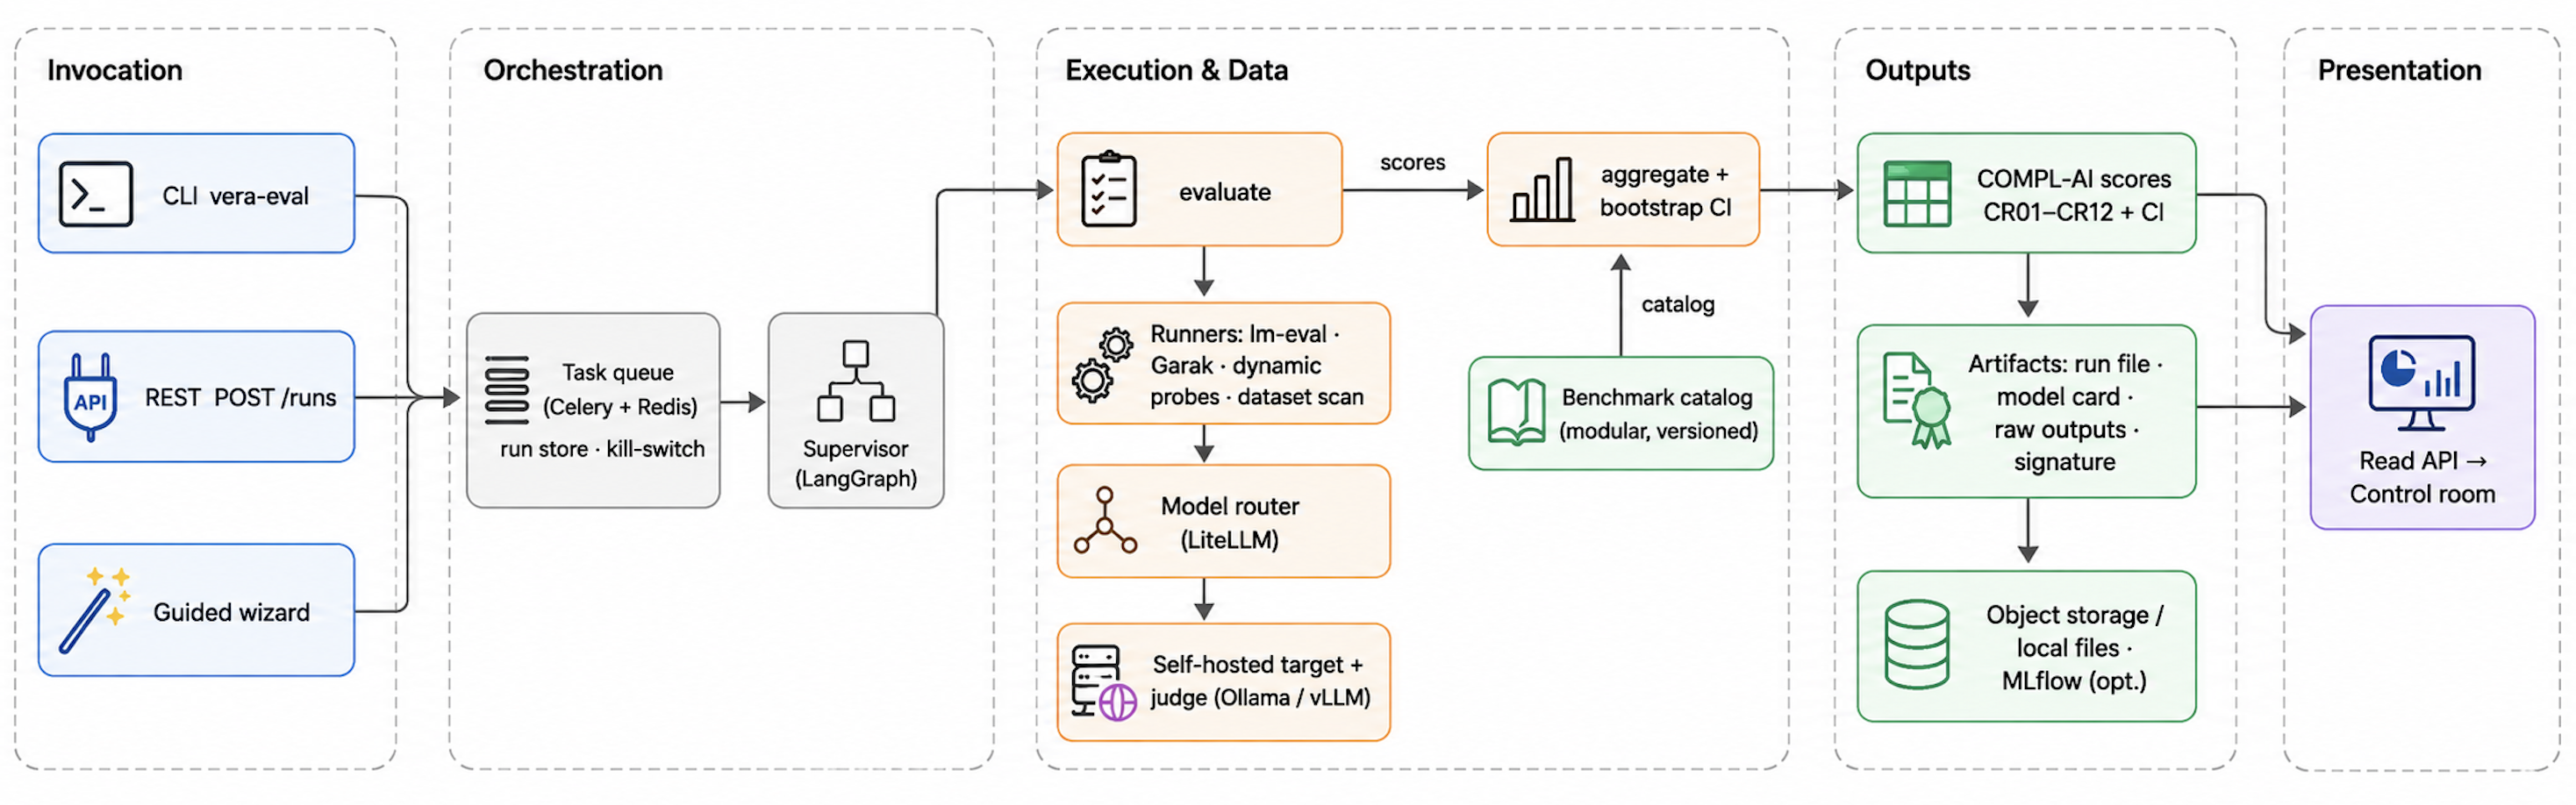
\includegraphics[width=\textwidth]{figures/fig2}
  \caption{Le pipeline d'exécution, regroupé en blocs. Trois surfaces d'invocation placent en file une même tâche déclarative ; un contrôleur en deux étapes exécute une étape \texttt{evaluate} (registre $\rightarrow$ exécuteurs $\rightarrow$ routeur de modèles $\rightarrow$ modèles auto-hébergés) et une étape \texttt{aggregate} qui combine les scores d'items mis en cache à l'aide du catalogue de benchmarks modulaire. Scores et artefacts transitent par une API de lecture vers le tableau de bord.}
  \label{fig:architecture}
\end{figure*}

\subsection{Piliers de l'IA responsable}
Après avoir montré comment le pipeline s'exécute, nous énonçons ce qu'il couvre.
Les piliers ne sont pas de notre choix : ce sont les six domaines de principes que COMPL-AI dérive des principes éthiques du règlement~\cite{guldimann2024complai,euaiact2024}, et le \Cref{tab:pillars} associe chacun aux exigences que VERA couvre et aux composants qui les évaluent.
La distinction entre modèle et système traverse le tableau : les exigences mesurables vérifient le modèle isolément, ce qui correspond aussi au périmètre déclaré de COMPL-AI, tandis que les exigences N et les artefacts liés à l'exécution adressent le système environnant, dont le règlement régule in fine la conformité.
La transparence couvre bien l'explicabilité : sa part mesurable comprend les capacités (CR06), la calibration et l'interprétabilité (CR07), la divulgation du caractère IA (CR08) et la traçabilité (CR09), mais juger une explication réelle résiste encore à l'automatisation.
VERA achemine donc l'explicabilité (N01) et la corrigibilité (N02) vers une revue humaine documentée, et les regroupe sous le pilier agentivité et supervision humaines, celui que COMPL-AI laisse sans exigence technique parce qu'il relève du niveau système.
C'est ce pilier qui maintient l'humain dans la boucle : la file de revue, les vues par rôles et le coupe-circuit (\Cref{sec:dashboard}) en constituent la surface opérationnelle.

\begin{table}[t]
  \caption{Les six piliers d'IA responsable couverts par VERA, les exigences COMPL-AI que VERA regroupe sous chacun (CR mesurables ; N revues par un humain ou déclaratives), et les composants qui les évaluent.}
  \label{tab:pillars}
  \centering
  \tblsetup
  \begin{tabularx}{\columnwidth}{@{}lcX@{}}
    \toprule
    Pilier & Exigences & Évalué par \\
    \midrule
    Agentivité \& supervision humaines & N01--N02 & file de revue humaine sur grille \\
    Robustesse \& sécurité & CR01--CR02 & exécuteur R01, Garak, \texttt{hf\_dynamic} \\
    Vie privée \& gouvernance des données & CR03--CR05 & \texttt{dataset\_scan}, Presidio \\
    Transparence & CR06--CR09, N04--N06 & \texttt{lm\_eval}, calibration, card/datasheet \\
    Diversité \& équité & CR10--CR12 & \texttt{hf\_bbq}, exécuteurs R11/R12 \\
    Sociétal \& environnemental & N03 & sondes énergétiques (CodeCarbon) \\
    \bottomrule
  \end{tabularx}
\end{table}

\subsection{Provenance des benchmarks}
Le catalogue (\texttt{benchmarks\_catalog.yaml}) définit, par exigence, quels benchmarks publics contribuent et avec quels poids ; il est versionné, de sorte qu'un changement de pondération est une nouvelle révision comparable plutôt qu'une modification de code.
C'est un artefact versionné et signé : chaque exécution épingle l'empreinte SHA-256 du catalogue à côté de ses scores, si bien qu'un score consigne la pondération exacte qui l'a produit.
Un benchmark sans poids au catalogue est exclu de l'agrégat plutôt que doté silencieusement d'une valeur par défaut, et la correspondance registre-catalogue est validée au démarrage de l'exécution, de sorte que chaque agrégat se reproduit exactement à partir de sa décomposition.
Chaque sortie par item consigne quel benchmark et quel exécuteur l'a produite.
Un indicateur explicite marque le cas où un moteur optionnel était absent et où un contrôle plus simple a été exécuté, afin qu'un lecteur puisse voir d'où vient chaque nombre.

\subsection{Moteurs au stade des données}
Les analyses de jeux de données renseignent CR03--CR05 dans le graphe : toxicité via Detoxify~\cite{hanu2020detoxify}, droits d'auteur via des heuristiques de mémorisation, et vie privée via la détection de données personnelles de Presidio~\cite{microsoft2023presidio}.
Elles s'exécutent sur le corpus synthétique de \Cref{sec:generated}.
Une évaluation de points de contrôle et un laboratoire d'empoisonnement de données existent également dans la plateforme mais sortent du périmètre de cet article (\Cref{app:lifecycle}).

\begin{figure*}[!t]
  \centering
  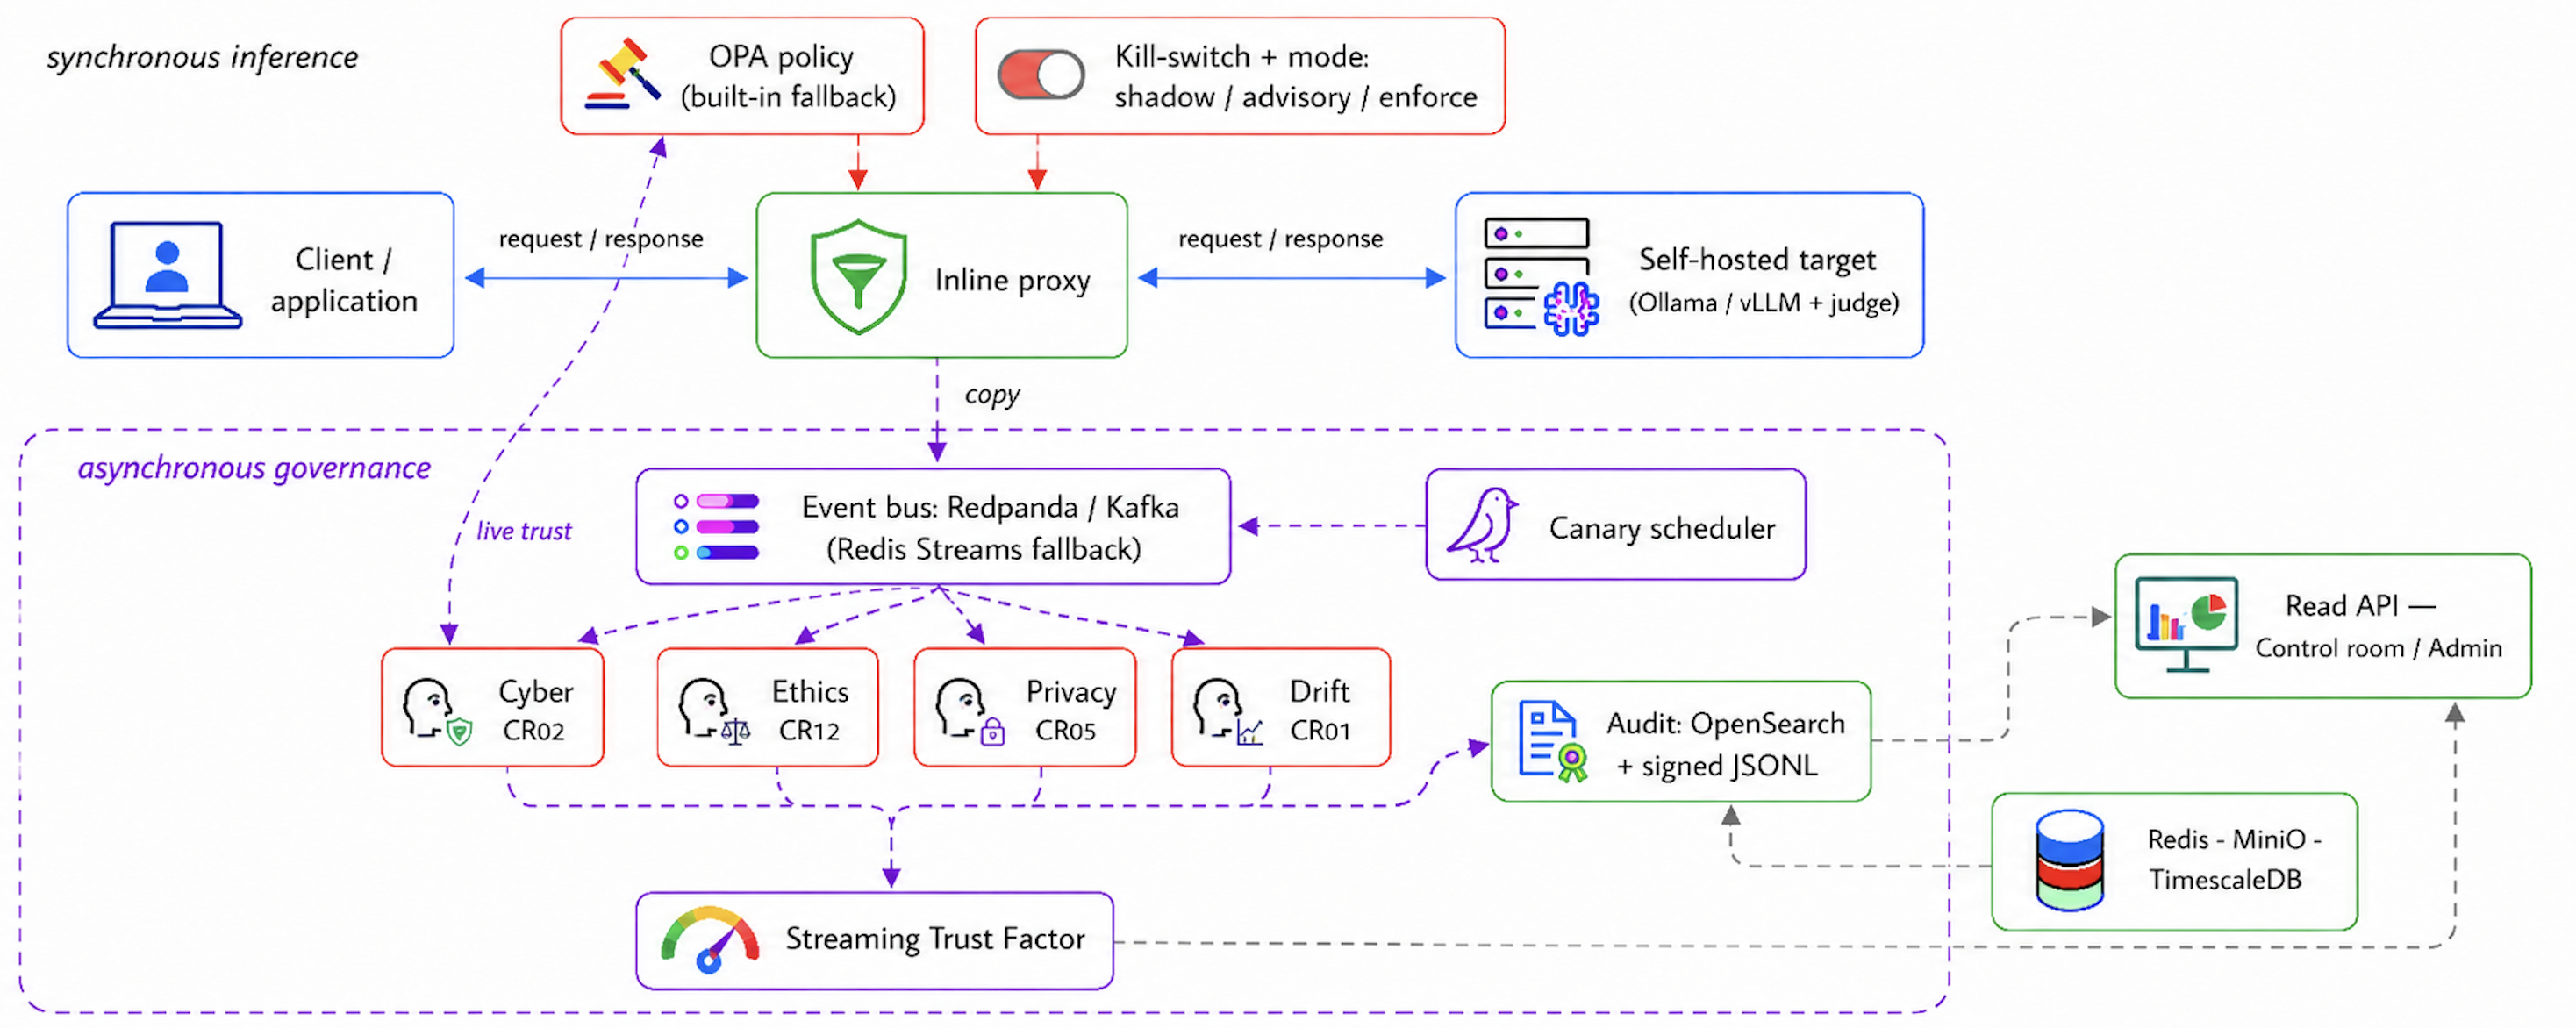
\includegraphics[width=\textwidth]{figures/fig3}
  \caption{La surcouche optionnelle de gouvernance à l'exécution. \emph{En haut :} le chemin synchrone : client, proxy en ligne et cible auto-hébergée, contrôlés par une décision de politique et par le coupe-circuit/mode. \emph{En bas :} la voie asynchrone : le proxy recopie le trafic vers un bus d'événements ; quatre agents (cyber, éthique, vie privée, dérive) le notent en un Trust Factor continu qui réalimente la politique ; chaque événement est signé pour l'audit, et chaque service externe se dégrade gracieusement vers un équivalent local.}
  \label{fig:gaas}
\end{figure*}

\subsection{Génération des artefacts de gouvernance}
Chaque exécution laisse une trace documentaire.
Les model cards suivent le format Model Cards~\cite{mitchell2019modelcard} : douze lignes mesurables, les statuts non mesurables, les URI d'évaluation de jeux de données, la provenance des benchmarks, les signatures et les limites.
Les datasheets~\cite{gebru2021datasheets} s'attachent aux analyses de corpus.
Des sondes environnementales consignent l'énergie et les émissions par exécution pour N03.
Un export d'audit signé rassemble l'état complet N01--N06 : les résultats de revue en direct pour N01 et N02, l'énergie mesurée et les formulaires attestés.

\subsection{Implémentation et profils de déploiement}
Le paquet \texttt{vera} vise Python~3.11 et livre trois profils de déploiement sur une seule base de code : une pile \emph{lite} en une commande (Redis, API, worker et un tableau de bord Next.js, artefacts locaux, sans authentification) ; une pile \emph{entreprise} complète en Docker Compose (ajoutant Keycloak RBAC, MLflow, MinIO, TimescaleDB) ; et une surcouche optionnelle de gouvernance à l'exécution qui supervise en direct un modèle déployé (proxy en ligne, couche de politique, coupe-circuit).
La surcouche (\Cref{fig:gaas}) place un proxy en ligne devant la cible ; quatre agents asynchrones notent le trafic en un Trust Factor en direct, et une couche de politique le transforme en décisions d'autorisation, de signalement ou de blocage.
Lors d'essais internes, elle a fonctionné en modes observation et consultatif ; le mode consultatif, qui signale les réponses peu fiables sans bloquer, correspondait à la cadence de contrôle interne de l'institution, et le coupe-circuit en un clic donne au responsable conformité un arrêt immédiat.
Son évaluation détaillée sort du périmètre de cet article.
Chaque couche se dégrade gracieusement : l'absence de MinIO ou de MLflow bascule vers des artefacts locaux et l'absence de suivi, de sorte que des déploiements partiels fonctionnent encore.
Le front-end du tableau de bord (\Cref{sec:dashboard}) consomme une API de lecture dédiée et un plan de contrôle d'administration.
La plateforme est validée par 143 tests unitaires backend et une matrice Playwright de 38 cas (accès par rôles, surfaces guidées, panneau de revue humaine, panneau de gouvernance, bascule de langue et module d'étude) ; le chemin optionnel \texttt{VERA\_E2E\_OLLAMA} rejoue une exécution complète.

\section{La salle de pilotage VERA}
\label{sec:dashboard}
Le tableau de bord constitue la contribution C1 : il transforme les scores d'exigences en une vue qu'un non-spécialiste peut lire, selon le principe « vue d'ensemble d'abord, zoom et filtrage, détails à la demande »~\cite{shneiderman1996eyes}.

\paragraph{Le score en un coup d'œil}
La synthèse s'ouvre sur une vue d'accueil délibérément épurée plutôt que sur un mur de tableaux (\Cref{fig:dashboard}).
Une jauge semi-circulaire place le Trust Factor sur trois segments alignés sur les seuils de bandes (rouge en dessous de 0,40, ambre jusqu'à 0,70, vert au-delà), à côté des comptes de verdicts et des exigences les plus faibles.
Le reste du détail, métadonnées d'exécution, provenance des benchmarks et tendances, reste à un clic derrière des sections repliées, de sorte que le premier écran ne porte que l'information sur laquelle repose une décision de mise en production.
Les écrans complets, y compris la vue détaillée dépliée, figurent en \Cref{app:dashboard}.

\paragraph{Triage par statut d'abord}
Le tableau des exigences est trié par état (échec, repli, non couvert, ok, n/a) plutôt que par identifiant, de sorte que la preuve la plus faible remonte en premier, et les lignes qui passent se replient derrière un contrôle « tout afficher ».
Les scores sont affichés en bandes verte, ambre et rouge, et non en succès/échec binaire, car les décisions de mise en production sont des arbitrages humains plutôt que des falaises de seuil.

\paragraph{Expliquer un score}
C'est la contribution C2.
Chaque ligne affiche un score, un intervalle et une justification en une ligne.
Cliquer sur une ligne ouvre un tiroir avec les benchmarks publics contributeurs, la model card et un exemple de sortie, de sorte qu'un lecteur voit \emph{pourquoi} une exigence est faible, et pas seulement qu'elle l'est.
Un inspecteur d'exécution expose le fichier d'exécution, le SHA git, la signature et la provenance par benchmark.

\paragraph{Graphiques}
Une courbe de tendance n'est tracée que lorsqu'au moins deux exécutions du même modèle existent ; sinon le tableau de bord affiche une seule bande de couverture.
Il ne fabrique pas une série temporelle à partir d'un point unique.

\paragraph{Vues par rôles et mode guidé}
Trois vues (IA responsable, cyber et data science) filtrent l'ensemble des exigences par rôle, avec une vue direction qui masque les détails internes.
Un mode guidé sans authentification est le comportement par défaut : un assistant en quatre étapes (choisir un modèle connecté, sélectionner un ensemble d'exigences recommandé ou personnalisé, régler les options, relire) soumet une exécution et ouvre une synthèse en direct.
C'est le chemin qu'emprunte un utilisateur non technique, tandis que les vues par rôles constituent la surface experte (\Cref{fig:dashboard} ; davantage d'écrans en \Cref{app:dashboard}).

\begin{figure*}[!t]
  \centering
  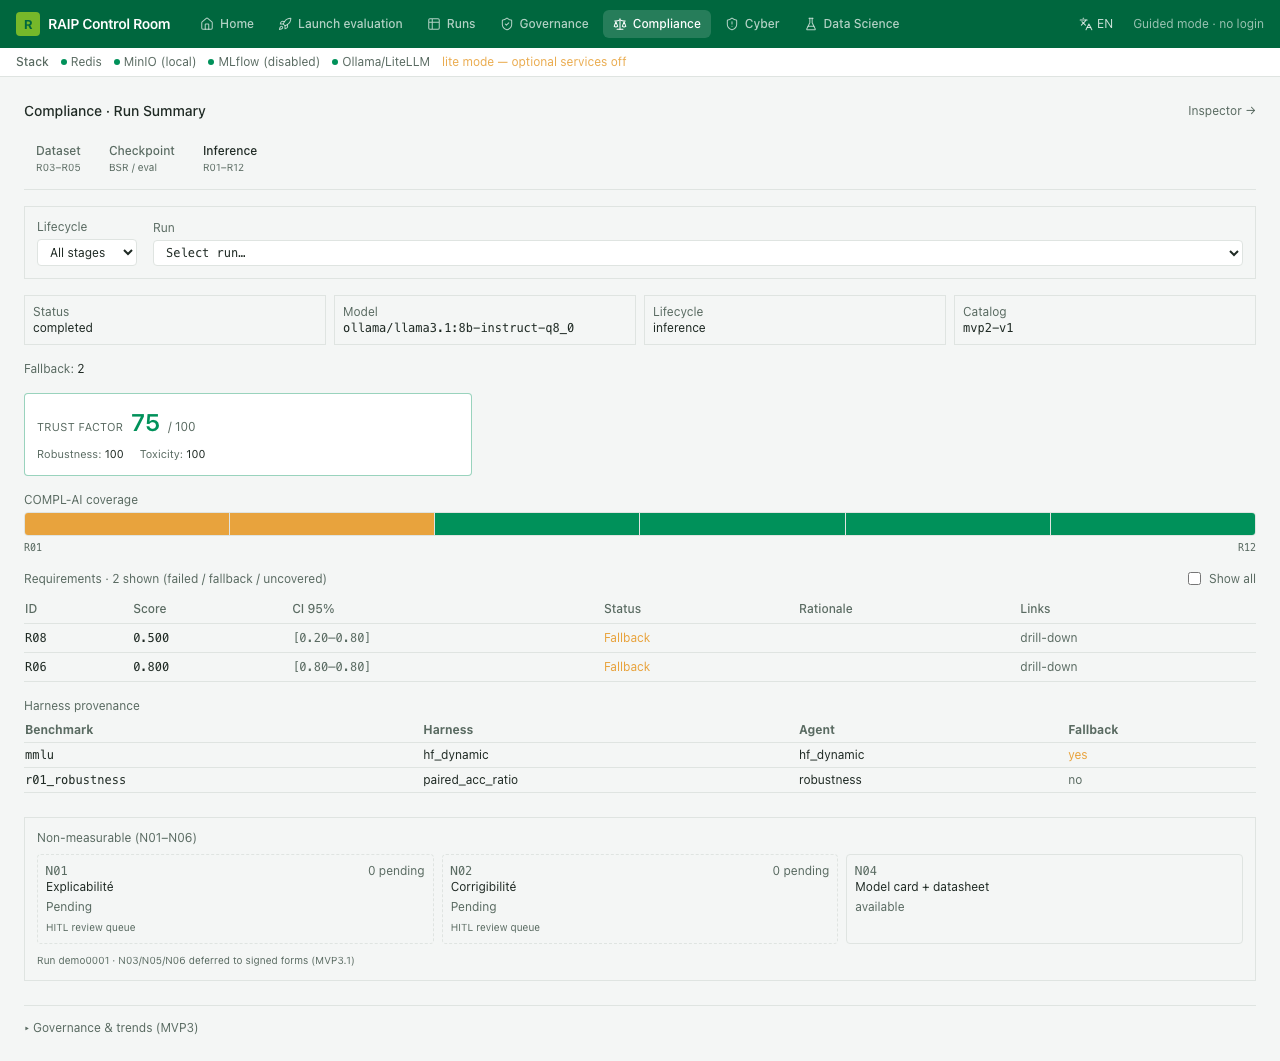
\includegraphics[width=0.92\textwidth]{figures/shot_control_room.png}
  \caption{La salle de pilotage VERA (mode guidé) sur une exécution d'évaluation. La vue d'accueil ne conserve que l'essentiel : la jauge du Trust Factor sur des segments alignés sur les bandes (rouge en dessous de 0,40, ambre jusqu'à 0,70, vert au-delà), les comptes de verdicts, les exigences les plus faibles et la bande de couverture par exigence ; le tableau de triage et les sections détaillées suivent en dessous (\Cref{app:dashboard}).}
  \label{fig:dashboard}
\end{figure*}

\section{Protocole d'évaluation}
\label{sec:evaluation}

\subsection{Questions de recherche}
Nous organisons l'évaluation autour de quatre questions pratiques, ce que nous voulions que l'outil fasse et s'il le fait, énoncées explicitement comme dans les travaux empiriques antérieurs en génie logiciel~\cite{liu2022mscpdp,weninger2018usecase}.
\begin{itemize}
  \item \emph{RQ1 (tableau de bord utilisable).} Un non-spécialiste peut-il piloter une exécution et en lire les résultats depuis le seul tableau de bord, sans écrire de code ? (C1)
  \item \emph{RQ2 (scores explicables).} VERA montre-t-il \emph{pourquoi} une exigence est faible, en décomposant le score entre critères et benchmarks publics sous-jacents ? (C2)
  \item \emph{RQ3 (couverture modulaire).} Un même framework évalue-t-il les douze exigences à travers différentes familles et tailles de modèles, et s'adapte-t-il à une autre spécification sans changement de code ? (C3, C4)
  \item \emph{RQ4 (robustesse des verdicts).} Dans quelle mesure le verdict de chaque exigence dépend-il de la pondération d'agrégation, et quels verdicts y sont invariants ? (C3)
\end{itemize}

\subsection{Systèmes étudiés et procédure}
Nous exécutons deux panels de modèles à poids ouverts auto-hébergés, afin que le même framework soit éprouvé à travers les marques et à travers les tailles.
Le panel~A comporte trois familles à taille comparable : Llama~3.1~8B, Qwen2.5~7B et Gemma~2~9B.
Le panel~B comporte une famille sur trois tailles : Ministral~3B, Mistral~7B et Mistral-Small~24B.
Un juge Llama~3.1~8B note les sondes de refus et de contournement.
Nous évaluons les douze exigences mesurables CR01--CR12 avec la graine~42 et $n{=}10$ items par benchmark.
Les six exigences non mesurables N01--N06 suivent le processus de revue humaine et d'attestation plutôt qu'un scoring automatisé, et n'apparaissent donc pas dans les tableaux de résultats.
Les exigences au stade des données CR03--CR05 s'exécutent sur le corpus synthétique de \Cref{sec:generated}, et sont donc identiques d'un modèle à l'autre.
Le \Cref{tab:datasets} liste le jeu de données public derrière chaque benchmark.

\emph{Note sur le service d'inférence.} Le point de terminaison de chat d'Ollama n'expose pas les log-probabilités de tokens, de sorte que les tâches de vraisemblance (capacité CR06, biais CR10) basculent vers les sondes dynamiques de VERA, consignées dans la provenance.
La sonde de sécurité \texttt{decodingtrust\_adv} bascule de même sur Apple Silicon.
Les moteurs CR03--CR05 et CR12 sont pleinement natifs sur n'importe quel backend.

\emph{Provenance de l'agrégation.} La pondération réside dans un catalogue versionné et signé dont l'empreinte SHA-256 est épinglée dans chaque exécution, de sorte que chaque score nomme la pondération exacte qui l'a produit.
Pour RQ4, une seule commande réagrège les mêmes résultats par benchmark mis en cache sous des pondérations alternatives, sans nouvelle interrogation des modèles ; l'étude est exactement reproductible à partir des artefacts publiés.

\begin{table}[t]
  \caption{Jeux de données publics derrière les exigences mesurables. CR03--CR05 utilisent le corpus synthétique de \Cref{sec:generated} plutôt qu'un jeu de données public ; CR08 utilise des sondes de divulgation dynamiques.}
  \label{tab:datasets}
  \centering
  \tblsetup
  \begin{tabularx}{\columnwidth}{@{}l l X@{}}
    \toprule
    Métrique & ID & Jeu(x) de données public(s) \\
    \midrule
    Robustesse & CR01 & MMLU~\cite{hendrycks2021mmlu} (perturbé) \\
    Résilience cyber & CR02 & AdvBench, DecodingTrust~\cite{wang2023decodingtrust} \\
    Capacités & CR06 & MMLU~\cite{hendrycks2021mmlu}, GSM8K~\cite{cobbe2021gsm8k}, HumanEval~\cite{chen2021humaneval}, TruthfulQA~\cite{lin2022truthfulqa}, BBH~\cite{suzgun2023bbh} \\
    Calibration & CR07 & MMLU~\cite{hendrycks2021mmlu} (confiance) \\
    Tatouage & CR09 & aucun ; test statistique~\cite{kirchenbauer2023watermark} \\
    Biais de représentation & CR10 & BBQ~\cite{parrish2022bbq}, BOLD~\cite{dhamala2021bold}, StereoSet~\cite{nadeem2021stereoset} \\
    Équité & CR11 & DecodingTrust~\cite{wang2023decodingtrust} (Adult) \\
    Toxicité & CR12 & RealToxicityPrompts~\cite{gehman2020realtoxicity}, TruthfulQA~\cite{lin2022truthfulqa} \\
    \bottomrule
  \end{tabularx}
\end{table}

\section{Résultats et analyse}
\label{sec:results}

Nous rapportons une exécution des deux panels (graine~42, $n{=}10$).
Les nombres illustrent le reporting et le contraste entre modèles, non un état de l'art en capacité.

\subsection{RQ1 : lire une exécution depuis le tableau de bord}
Nous évaluons le tableau de bord au moyen d'une petite étude utilisateur auto-administrée, conduite à travers la plateforme elle-même.
Cinq chercheurs du laboratoire de recherche de l'institution hôte (aucun n'étant auteur, aucun n'ayant participé à la construction de VERA) ont réalisé huit tâches de lecture fixes en mode guidé (sans authentification) sur une exécution préchargée, accessible à distance via un déploiement partagé.
L'application a mesuré le temps par tâche avec une horloge monotone, validé chaque réponse côté serveur contre une clé figée à partir de l'exécution, et n'a jamais divulgué la justesse pendant une session ; les tâches étaient plafonnées à cinq minutes, sans animateur ni indice.
Les tâches couvrent le chemin de lecture de bout en bout : trouver l'exigence la plus faible, lire sa bande et son intervalle, identifier les replis, juger la couverture, atteindre un exemple de sortie, distinguer échec, repli et ok, lire le Trust Factor, et lancer une exécution (\Cref{fig:dashboard} ; \Cref{app:dashboard}).
Les participants ont accompli 38 des 40 tâches : l'un a mal identifié l'ensemble de repli à neuf benchmarks (T3, la tâche la plus difficile, qui demande un ensemble exact), et l'un a atteint le plafond de cinq minutes sur la tâche d'exemple de sortie (T5).
Le temps médian a été de 24\,s par tâche de lecture (IQ 15--42\,s), et de 92\,s pour lancer une exécution de bout en bout.
Le protocole, le module d'étude et le script d'analyse sont livrés avec le paquet de réplication.
Les participants étaient des chercheurs familiers de l'IA plutôt que des responsables conformité ; un panel avec des profils conformité et risques, assorti d'une mesure d'accord inter-annotateurs~\cite{hayes2007krippendorff,studtmann2023histree}, reste un travail futur.

\subsection{RQ2 : expliquer un score}
VERA ne s'arrête pas à un nombre.
Ouvrir une exigence faible montre ses benchmarks publics contributeurs et leurs scores individuels, de sorte que la cause est visible plutôt qu'inférée.
Par exemple, lorsqu'un modèle obtient un score bas sur le biais de représentation (CR10), le tiroir montre quel benchmark de biais l'a provoqué (BBQ, BOLD ou StereoSet), et le clic mène aux exemples de sorties.
Chaque score d'exigence est donc expliqué par la preuve publique qui le sous-tend, ce que demande RQ2.

\subsection{RQ3 : un seul framework à travers familles et tailles}
Le \Cref{tab:panelA} (familles) et le \Cref{tab:panelB} (tailles) rapportent les douze exigences pour les deux panels, calculées par le \emph{même} framework, sans changement de code entre les deux.
C'est l'étude reproductible C4, et l'exécuter à l'identique sur deux panels constitue la preuve de la revendication de modularité C3.
Nous avons également éprouvé cette revendication directement : une spécification alternative, un sous-ensemble orienté sécurité avec des benchmarks adverses surpondérés, est livrée sous forme de deux fichiers de données (registre et catalogue signé) et se charge par simple configuration.
Le pipeline inchangé l'a exécutée de bout en bout (graine~42) et a produit des verdicts en bandes sous le catalogue alternatif ; l'exécution et sa provenance figurent dans le paquet de réplication.
Une colonne se lit en trois étapes : choisir une exigence, lire sa bande, et l'ouvrir dans le tableau de bord pour atteindre le benchmark sous-jacent.
Les panels révèlent des différences entre modèles.
Sur le panel des familles, l'équité (CR11) sépare nettement les modèles : Qwen2.5 tombe à $0{,}00$ tandis que Llama et Gemma atteignent $1{,}00$, et la résilience cyber (CR02) ainsi que la toxicité (CR12) les distinguent aussi.
Sur le panel des tailles, la capacité (CR06) augmente avec l'échelle, de $0{,}70$ à 3B et 7B jusqu'à $1{,}00$ à 24B.
Pourtant le modèle 24B tombe à zéro sur l'équité (CR11 $=0{,}00$) et la résilience cyber (CR02 $=0{,}00$).
En observation annexe, les frameworks COMPL-AI et VERA nous montrent qu'un modèle plus grand n'est pas toujours un modèle plus responsable.
Ce sont là les écarts entre modèles qu'un lecteur souhaite repérer.
À $n{=}10$ items par benchmark, des écarts extrêmes tels que CR11 $0{,}00$ contre $1{,}00$ sont des signaux à investiguer, non des estimations précises ; les intervalles bootstrap sont livrés avec les artefacts d'exécution.
Les scores au stade des données CR03--CR05 sont identiques d'un modèle à l'autre, puisque les analyses portent sur le corpus et non sur le modèle : CR03 $=0{,}84$, CR04 $=0{,}94$ et CR05 $=0{,}73$ (Presidio détecte les données personnelles implantées).
Le tatouage CR09 vaut $0{,}00$ pour chaque modèle : le test statistique~\cite{kirchenbauer2023watermark} recherche un biais de liste verte à la Kirchenbauer, et les modèles ouverts ne portent pas un tel tatouage ; le score correct est donc zéro plutôt qu'un faux positif.

\begin{table}[t]
  \caption{Panel~A (familles) : les douze exigences mesurables pour trois familles de modèles à taille comparable (graine~42, $n{=}10$). Meilleur par ligne en \textbf{gras}. CR03--CR05 sont des analyses de corpus (indépendantes du modèle) ; CR09 vaut zéro pour tous les modèles ouverts non tatoués.}
  \label{tab:panelA}
  \centering
  \tblsetup
  \begin{tabularx}{\columnwidth}{@{}X l c c c@{}}
    \toprule
    Métrique & ID & Llama 3.1 8B & Qwen2.5 7B & Gemma 2 9B \\
    \midrule
    Robustesse & CR01 & 1,00 & 1,00 & 1,00 \\
    Résilience cyber & CR02 & \best{0,50} & 0,25 & 0,00 \\
    Adéquation des données & CR03 & 0,84 & 0,84 & 0,84 \\
    Droits d'auteur & CR04 & 0,94 & 0,94 & 0,94 \\
    Vie privée & CR05 & 0,73 & 0,73 & 0,73 \\
    Capacités & CR06 & 0,80 & 0,80 & 0,80 \\
    Calibration & CR07 & 0,90 & 0,90 & 0,90 \\
    Divulgation IA & CR08 & 0,50 & \best{1,00} & \best{1,00} \\
    Tatouage & CR09 & 0,00 & 0,00 & 0,00 \\
    Biais de représentation & CR10 & 0,67 & 0,67 & 0,67 \\
    Équité & CR11 & \best{1,00} & 0,00 & \best{1,00} \\
    Toxicité & CR12 & \best{0,75} & 0,62 & \best{0,75} \\
    \bottomrule
  \end{tabularx}
\end{table}

\begin{table}[t]
  \caption{Panel~B (tailles) : les mêmes douze exigences pour une famille (Mistral) sur trois tailles (graine~42, $n{=}10$). Meilleur par ligne en \textbf{gras}. CR03--CR05 sont des analyses de corpus ; CR09 vaut zéro pour tous.}
  \label{tab:panelB}
  \centering
  \tblsetup
  \begin{tabularx}{\columnwidth}{@{}X l c c c@{}}
    \toprule
    Métrique & ID & Ministral 3B & Mistral 7B & Mistral-Small 24B \\
    \midrule
    Robustesse & CR01 & 0,93 & \best{1,00} & 0,77 \\
    Résilience cyber & CR02 & \best{0,50} & \best{0,50} & 0,00 \\
    Adéquation des données & CR03 & 0,84 & 0,84 & 0,84 \\
    Droits d'auteur & CR04 & 0,94 & 0,94 & 0,94 \\
    Vie privée & CR05 & 0,73 & 0,73 & 0,73 \\
    Capacités & CR06 & 0,70 & 0,70 & \best{1,00} \\
    Calibration & CR07 & 0,90 & 0,90 & 0,90 \\
    Divulgation IA & CR08 & 1,00 & 1,00 & 1,00 \\
    Tatouage & CR09 & 0,00 & 0,00 & 0,00 \\
    Biais de représentation & CR10 & 0,33 & 0,33 & \best{0,67} \\
    Équité & CR11 & \best{1,00} & \best{1,00} & 0,00 \\
    Toxicité & CR12 & \best{0,75} & 0,60 & \best{0,75} \\
    \bottomrule
  \end{tabularx}
\end{table}

\subsection{RQ4 : dans quelle mesure le verdict dépend-il de la pondération ?}
\label{sec:rq4}
Chaque score d'exigence est une moyenne pondérée de ses moyennes par benchmark, $s_R(w)=\sum_{b\in B_R} w_b\, m_b$ avec $w_b\ge 0$ et $\sum_b w_b=1$, lue depuis le catalogue signé.
Le score est donc une combinaison convexe des $m_b$, ce qui produit un énoncé de robustesse en forme fermée.

\begin{proposition}[Plage atteignable sous repondération]
\label{prop:range}
Pour toute pondération admissible $w$, $\min_{b} m_b \le s_R(w) \le \max_{b} m_b$, et les deux bornes sont atteintes par les pondérations extrêmes (un seul benchmark).
Sur l'ensemble du simplexe des pondérations, la plage atteignable de $s_R$ est donc exactement $\Delta_R=\max_b m_b-\min_b m_b$.
\end{proposition}

Deux conséquences portent la valeur d'audit.
Si $\Delta_R=0$, ou si l'intervalle $[\min_b m_b,\max_b m_b]$ se situe à l'intérieur d'une seule bande, le verdict est \emph{invariant} : aucune repondération ne peut le faire basculer.
Si l'intervalle chevauche un seuil de bande ($0{,}40$ ou $0{,}70$), le verdict est \emph{dépendant des poids} : une repondération admissible le fait basculer.
Le \Cref{tab:sensitivity} et la \Cref{fig:sensitivity} rapportent $\Delta_R$ et l'indicateur de bascule pour chaque exigence multi-benchmarks sur les deux panels, calculés par une seule commande à partir des décompositions mises en cache, sans nouvelle interrogation des modèles.

Le résultat est non dégénéré, et il joue dans les deux sens.
Nous observons que la robustesse (CR01) est invariante sur chaque modèle : son verdict ne dépend pas de la pondération.
La capacité (CR06), le biais de représentation (CR10) et la toxicité (CR12) dépendent des poids sur la plupart des modèles ($\Delta{=}1{,}00$) : les mêmes résultats mis en cache s'agrègent en un verdict vert ou rouge par le seul choix des poids.
Sur le panel des tailles, le plus grand modèle inverse le schéma : son verdict de capacité devient invariant tandis que son verdict de biais reste dépendant des poids, ce qui appuie l'observation annexe selon laquelle un modèle plus grand n'est pas toujours plus responsable.
Un relecteur lit donc le \Cref{tab:panelA,tab:panelB} conjointement avec le \Cref{tab:sensitivity} : le premier donne les verdicts, le second dit lesquels survivraient à une pondération différente.
Un balayage empirique corrobore la borne au pire cas : sur 200 perturbations aléatoires des poids du catalogue, un bruit modéré ($\sigma{=}0{,}1$) fait déjà basculer $0{,}5$ bande par tirage en moyenne (jusqu'à deux), et un bruit plus fort ($\sigma{=}0{,}2$) réordonne le classement de triage du tableau de bord dans $64\%$ des tirages.

La borne change aussi les décisions entre politiques défendables, et pas seulement sous l'effet du bruit.
Nous avons réagrégé les résultats des panels mis en cache sous trois politiques nommées : la moyenne uniforme que fixe COMPL-AI, notre catalogue signé, et l'alternative « sécurité d'abord » livrée avec le framework, qui surpondère les benchmarks adverses.
Quatre verdicts sur trente basculent (\Cref{tab:policies}), tous sur la toxicité (CR12) : les mêmes résultats mis en cache se lisent verts sous la politique uniforme et ambre sous la politique « sécurité d'abord ».
Un nombre unique non pondéré rapporte le verdict vert sans divulguer cette dépendance ; le catalogue signé, conjointement avec la \Cref{prop:range}, la rend visible et auditable.

\begin{table}[t]
  \caption{Verdicts qui basculent entre trois politiques de pondération défendables, réagrégés à partir des mêmes moyennes par benchmark mises en cache (sans nouvelle interrogation des modèles). « Uniforme » est l'agrégation de COMPL-AI ; le catalogue « sécurité d'abord » est livré avec le paquet de réplication. v = vert, a = ambre.}
  \label{tab:policies}
  \centering
  \tblsetup
  \begin{tabularx}{\columnwidth}{@{}X l c c c@{}}
    \toprule
    Modèle & Métrique & Uniforme & Catalogue & Sécurité d'abord \\
    \midrule
    Llama 3.1 8B & Toxicité (CR12) & 0,750 (v) & 0,750 (v) & 0,600 (a) \\
    Gemma 2 9B & Toxicité (CR12) & 0,750 (v) & 0,750 (v) & 0,600 (a) \\
    Ministral 3B & Toxicité (CR12) & 0,746 (v) & 0,746 (v) & 0,697 (a) \\
    Mistral-Small 24B & Toxicité (CR12) & 0,750 (v) & 0,750 (v) & 0,600 (a) \\
    \bottomrule
  \end{tabularx}
\end{table}

\begin{table}[t]
  \caption{Plage atteignable $\Delta_R$ sous toute repondération admissible et possibilité de bascule de la bande du verdict (\Cref{prop:range}), par exigence multi-benchmarks ($k$ = benchmarks contributeurs). $\Delta{=}0$ indique que le verdict est invariant à la pondération ; « bascule » signale une dépendance aux poids.}
  \label{tab:sensitivity}
  \centering
  \tblsetup
  \begin{tabularx}{\columnwidth}{@{}l c *{3}{>{\centering\arraybackslash}X}@{}}
    \toprule
    \multicolumn{5}{@{}l}{\emph{Panel A (familles)} : Llama 3.1 8B / Qwen2.5 7B / Gemma 2 9B} \\
    \midrule
    Robustesse (CR01) & 3 & $\Delta{=}0{,}00$, non & $\Delta{=}0{,}00$, non & $\Delta{=}0{,}00$, non \\
    Résilience cyber (CR02) & 4 & $\Delta{=}1{,}00$, bascule & $\Delta{=}1{,}00$, bascule & $\Delta{=}0{,}00$, non \\
    Capacités (CR06) & 5 & $\Delta{=}1{,}00$, bascule & $\Delta{=}1{,}00$, bascule & $\Delta{=}1{,}00$, bascule \\
    Biais de repr. (CR10) & 3 & $\Delta{=}1{,}00$, bascule & $\Delta{=}1{,}00$, bascule & $\Delta{=}1{,}00$, bascule \\
    Toxicité (CR12) & 4 & $\Delta{=}1{,}00$, bascule & $\Delta{=}1{,}00$, bascule & $\Delta{=}1{,}00$, bascule \\
    \midrule
    \multicolumn{5}{@{}l}{\emph{Panel B (tailles)} : Ministral 3B / Mistral 7B / Mistral-Small 24B} \\
    \midrule
    Robustesse (CR01) & 3 & $\Delta{=}0{,}30$, non & $\Delta{=}0{,}00$, non & $\Delta{=}0{,}30$, non \\
    Résilience cyber (CR02) & 4 & $\Delta{=}1{,}00$, bascule & $\Delta{=}1{,}00$, bascule & $\Delta{=}0{,}00$, non \\
    Capacités (CR06) & 5 & $\Delta{=}1{,}00$, bascule & $\Delta{=}1{,}00$, bascule & $\Delta{=}0{,}00$, non \\
    Biais de repr. (CR10) & 3 & $\Delta{=}1{,}00$, bascule & $\Delta{=}1{,}00$, bascule & $\Delta{=}1{,}00$, bascule \\
    Toxicité (CR12) & 4 & $\Delta{=}0{,}52$, bascule & $\Delta{=}1{,}00$, bascule & $\Delta{=}1{,}00$, bascule \\
    \bottomrule
  \end{tabularx}
\end{table}

\begin{figure}[t]
  \centering
  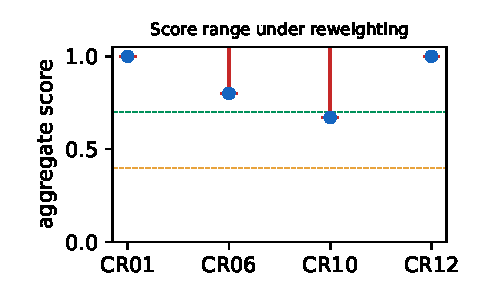
\includegraphics[width=0.80\columnwidth]{figures/fig_weight_sensitivity.pdf}
  \caption{Agrégat de référence (point) et plage atteignable sous toute repondération (barre) par exigence multi-benchmarks, pour les deux panels. Les lignes pointillées marquent les seuils de bandes ; une barre qui franchit une ligne correspond à un verdict dépendant des poids.}
  \label{fig:sensitivity}
\end{figure}

\subsection{Limites}
L'étude utilisateur est de petite taille ($n{=}5$) et ses participants étaient des chercheurs du laboratoire de l'institution hôte, familiers de l'IA plutôt que profils conformité ; la revendication « non-spécialiste » repose donc sur la conception plus ce premier essai. Un modèle juge (Llama~3.1~8B) peut par ailleurs biaiser les sondes jugées par LLM.
CR06 et CR10 utilisent des sondes dynamiques sous la contrainte de log-probabilités d'Ollama plutôt qu'un scoring natif par vraisemblance ; c'est consigné dans la provenance, et un backend vLLM permettrait au chemin natif de corroborer ces scores.
Les panels couvrent des modèles à poids ouverts de 3B à 24B avec $n{=}10$ items par benchmark et une seule graine ; des modèles plus grands, davantage d'items ou davantage de graines pourraient déplacer les nombres.
Nous présentons l'étude comme une illustration de la méthode, non comme un large benchmark empirique ; le protocole signé, exécutable en une commande, rend ces extensions mécaniques.
Comme COMPL-AI, VERA ne score pas automatiquement les six exigences non mesurables ; sa contribution y est un chemin traçable de revue humaine et d'attestation, non une nouvelle métrique, et les tableaux de panels ne rapportent que les douze exigences mesurables.
Les poids du catalogue sont conçus par les auteurs ; la \Cref{prop:range} borne l'effet de leur repondération, non celui de la sélection de benchmarks différents.
Les scores COMPL-AI sont des approximations techniques d'obligations réglementaires~\cite{guldimann2024complai,euaiact2024}, non des conclusions juridiques, et les bandes sont des aides au jugement humain, non des barrières automatiques.
Savoir si un déploiement donné relève des obligations du règlement, et de quelle manière, demeure une question juridique propre à chaque juridiction ; cet article fournit un socle technique, non une interprétation juridique.
Le banc d'essai du runtime de gouvernance mesure la surcharge par requête et la détection sur des cas implantés, non une charge de production soutenue.

\section{Données générées et application bancaire}
\label{sec:application}
Cette section couvre deux compléments au benchmark de modèles : le corpus synthétique que nous générons pour les exigences au stade des données, et un cadre de déploiement réglementé qui illustre comment la même exécution est lue par un relecteur sectoriel.

\subsection{Données générées}
\label{sec:generated}
Les exigences au stade des données CR03--CR05 s'exécutent sur un corpus entièrement synthétique : nous avons généré chaque document, et aucune donnée réelle de client ou d'institution n'a été utilisée.
Un générateur à graine fixe produit 230 documents bancaires courts, publiés sous le nom \texttt{banking\_synth.jsonl} (dossiers FR/EN de banque de détail, entreprise, gestion de patrimoine et réclamations), qui implantent les modes de défaillance que le stade des données doit détecter : IBAN synthétiques (\texttt{FR76} suivi de 23 chiffres), RIB, adresses e-mail et numéros de téléphone pour la vie privée ; paires quasi dupliquées pour les droits d'auteur ; et segments de clientèle déséquilibrés pour l'adéquation des données.
Les moteurs natifs obtiennent alors vie privée CR05 $=0{,}73$ (rappel de Presidio sur les données personnelles implantées), droits d'auteur CR04 $=0{,}94$ (détection de quasi-doublons par Levenshtein et BLEU) et adéquation des données CR03 $=0{,}84$ (heuristiques d'équilibre entre groupes).
Comme les analyses portent sur le corpus et non sur le modèle, ces scores sont indépendants du modèle, et le générateur (\texttt{gen\_banking\_corpus.py}) les rend entièrement reproductibles.

\subsection{Application en banque}
VERA est générique : les modèles qu'il évalue sont à usage général, non spécifiques à la banque, et le framework l'est également.
La banque est donc une illustration d'usage dans un secteur réglementé, non le périmètre du framework.
Considérons un point de contrôle avant mise en production pour un assistant de banque de détail (FAQ sur les comptes, explication de produits, tri des réclamations).
Sous l'approche par les risques du règlement, un tel assistant n'est pas un système à haut risque : il relève des obligations de transparence de l'art.~50, tandis que l'usage bancaire que le règlement classe à haut risque (annexe~III) est l'évaluation de solvabilité.
Les exigences contraignantes qui pèsent sur l'assistant proviennent en revanche des obligations de contrôle interne et de risque de modèle de la banque, qu'une seconde ligne de défense suit déjà : DORA~\cite{dora2022}, les orientations TIC de l'EBA~\cite{eba2021ictrisk} et les travaux de l'ACPR sur l'IA en finance~\cite{acpr2020ai} ; la \Cref{app:banking} donne la correspondance détaillée.
La même exécution produit donc des preuves techniques que ces contrôles internes peuvent consommer, et des artefacts qu'un relecteur bancaire reconnaît.

\section{Enseignements tirés}
\label{sec:lessons}
Construire et exploiter VERA au sein d'une institution réglementée nous a appris cinq leçons qui se transposent au-delà de ce framework.

\textbf{Un score global unique est un piège en pratique.}
La politique d'agrégation s'est révélée être un choix de gouvernance, non un détail technique : quatre verdicts sur trente basculent entre deux pondérations défendables (\Cref{tab:policies}), sur les mêmes résultats mis en cache.
La politique doit être visible, signée et contestable, sinon le verdict encode silencieusement les préférences non examinées de quelqu'un.

\textbf{La spécification doit être une donnée, pas du code.}
Une version antérieure codait en dur le chemin du catalogue, et notre revendication de modularité devançait le code.
Externaliser le registre et le catalogue signé en configuration a rendu la revendication testable, et a rendu chaque politique de scoring auditable par simple comparaison de versions.

\textbf{Les non-spécialistes n'adoptent pas les lignes de commande.}
Le tableau de bord guidé et sans authentification est né de l'observation de responsables conformité et risques se détournant des flux en ligne de commande ; c'est l'opérabilité, et non la visualisation, qui a porté l'adoption.

\textbf{La dégradation gracieuse est une exigence de déploiement, pas un agrément.}
Les environnements réels manquent de log-probabilités de tokens, de moteurs optionnels ou de noyaux GPU ; des indicateurs de repli explicites ont maintenu les exécutions honnêtes là où une dégradation silencieuse aurait corrompu la preuve.

\textbf{Les artefacts liés à l'exécution suppriment une friction d'audit réelle.}
Une documentation rédigée après coup dérive de l'évaluation qu'elle décrit ; générer la model card et la datasheet à partir de l'exécution elle-même a rendu cette dérive structurellement impossible.

\section{Conclusion et travaux futurs}
\label{sec:conclusion}

L'EU AI Act demande aux organisations des preuves techniques sur l'ensemble des principes de l'IA de confiance.
COMPL-AI a traduit le règlement en dix-huit exigences techniques et a évalué les douze mesurables sur des jeux de données publics.
VERA franchit l'étape suivante et transforme cette référence en un framework opérationnel.
Il exécute les mêmes douze exigences sur des jeux de données publics et un corpus synthétique publié.
Il rend la politique de scoring signée et auditable, et rapporte quels verdicts sont robustes à une repondération.
Il émet des artefacts de preuve liés à l'exécution et achemine les six exigences non mesurables vers un chemin humain traçable.
Aucun outil voisin ne réunit ces propriétés : HELM et lm-eval standardisent la mesure, COMPL-AI fige une pondération implicite, et aucun d'eux ne conditionne le résultat pour un non-spécialiste.
Nous apportons une première preuve, issue d'une petite étude utilisateur auto-administrée, qu'un lecteur peut piloter une exécution depuis le seul tableau de bord (RQ1), et chaque verdict se décompose en la preuve publique qui le sous-tend (RQ2).
Nous rapportons en outre qu'un même framework couvre les douze exigences à travers familles et tailles de modèles sans changement de code (RQ3), et que la dépendance de chaque verdict à la pondération est bornée en forme fermée (RQ4).
Sur les deux panels, VERA signale des écarts concrets d'IA responsable, et met en évidence une exigence de tatouage qu'aucun modèle ouvert ne satisfait.
Nous publions VERA en logiciel open-source, disponible à l'adresse \url{\repourl}, afin d'accélérer l'adoption et de diffuser les bonnes pratiques d'IA responsable.
Les travaux futurs comprennent une étude formelle auprès de praticiens avec mesure d'accord inter-annotateurs~\cite{hayes2007krippendorff,studtmann2023histree}, des exécutions natives par log-probabilités sur un backend vLLM, et le scoring par rôle et par persona que cet article, centré sur le logiciel, ne fait qu'esquisser.

{\footnotesize
\bibliographystyle{IEEEtran}
\bibliography{references}
}

\appendices

\section{Extensions de laboratoire sur le cycle de vie}
\label{app:lifecycle}
Au-delà des stades d'inférence et de données exercés dans le corps de l'article, la plateforme comprend deux extensions de cycle de vie hors périmètre : un évaluateur de points de contrôle qui écrit des séries temporelles par métrique au fil des points de contrôle d'entraînement, et un laboratoire d'empoisonnement de données qui injecte des portes dérobées et rapporte un taux de survie pour la résilience cyber (CR02).
Les deux réutilisent les exécuteurs et le catalogue du chemin d'inférence.

\section{Correspondance réglementaire bancaire}
\label{app:banking}
Le \Cref{tab:banking-map} associe les six mêmes piliers que le \Cref{tab:pillars} aux obligations du secteur bancaire qu'une seconde ligne de défense suit déjà, de sorte que la même exécution produit des artefacts qu'un relecteur bancaire reconnaît.

\begin{table}[h]
  \caption{L'exécution de contrôle avant mise en production associe les six piliers du \Cref{tab:pillars} (via les exigences COMPL-AI) aux obligations du secteur bancaire.}
  \label{tab:banking-map}
  \centering
  \tblsetup
  \begin{tabularx}{\columnwidth}{@{}l l X@{}}
    \toprule
    Pilier & Exigence VERA & Obligation bancaire \\
    \midrule
    Agentivité \& supervision humaines & N01--N02 & supervision humaine / double regard ACPR~\cite{acpr2020ai} \\
    Robustesse \& sécurité & CR01--CR02 & risque TIC \& tests de résilience DORA~\cite{dora2022} ; EBA~\cite{eba2021ictrisk} \\
    Vie privée \& gouv. des données & CR03--CR05 & contrôles de données connexes au RGPD ; qualité \& sécurité des données EBA~\cite{eba2021ictrisk} \\
    Transparence & CR06--CR09, N04--N06 & explicabilité \& traçabilité ACPR~\cite{acpr2020ai} \\
    Diversité \& équité & CR10--CR12 & non-discrimination en finance ACPR~\cite{acpr2020ai} \\
    Sociétal \& environnemental & N03 & reporting énergétique (CodeCarbon, mesuré) \\
    \bottomrule
  \end{tabularx}
\end{table}

\section{Écrans du tableau de bord}
\label{app:dashboard}
Les \Cref{fig:app-home,fig:app-wizard,fig:app-gov,fig:app-full} montrent, en taille réelle, les écrans qui sous-tendent la vue d'accueil de la \Cref{fig:dashboard} : l'accueil en mode guidé, l'assistant de lancement en quatre étapes, le panneau de gouvernance, et la vue complète d'une exécution avec ses sections de détail dépliées (triage, bandeau des exigences non mesurables, métadonnées d'exécution et provenance des exécuteurs).

\begin{figure*}[p]
  \centering
  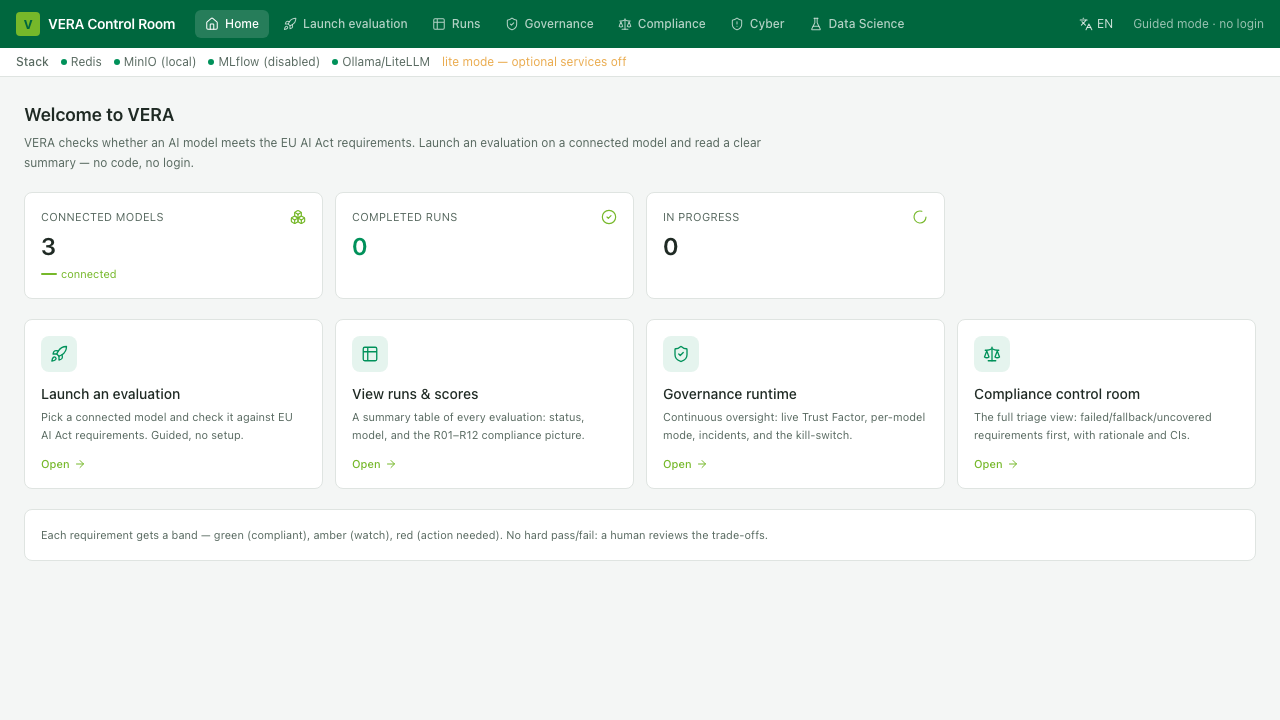
\includegraphics[width=\textwidth,height=0.42\textheight,keepaspectratio]{figures/shot_home.png}
  \caption{L'accueil en mode guidé : actions de prise en main, modèles connectés, état de la pile technique et coupe-circuit, sans authentification requise.}
  \label{fig:app-home}
\end{figure*}

\begin{figure*}[p]
  \centering
  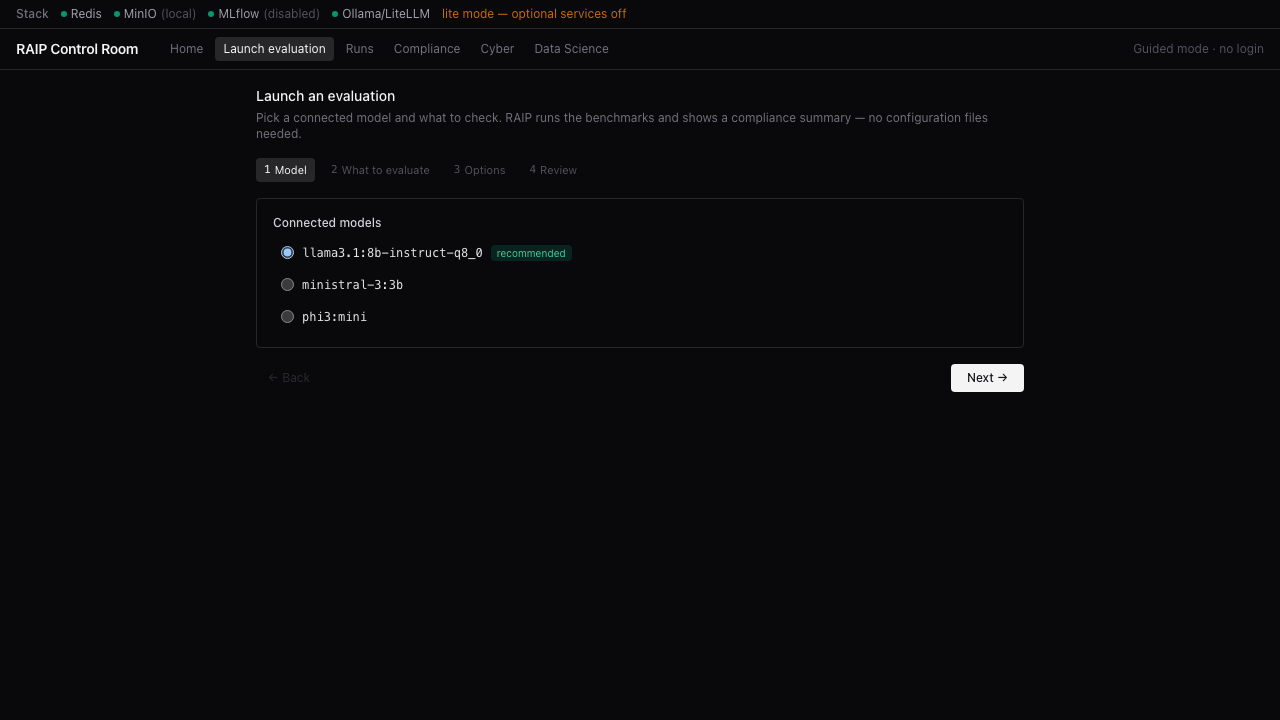
\includegraphics[width=\textwidth,height=0.42\textheight,keepaspectratio]{figures/shot_wizard.png}
  \caption{L'assistant de lancement en quatre étapes : choisir un modèle connecté, sélectionner un ensemble d'exigences recommandé ou personnalisé, régler les options, relire et soumettre.}
  \label{fig:app-wizard}
\end{figure*}

\begin{figure*}[p]
  \centering
  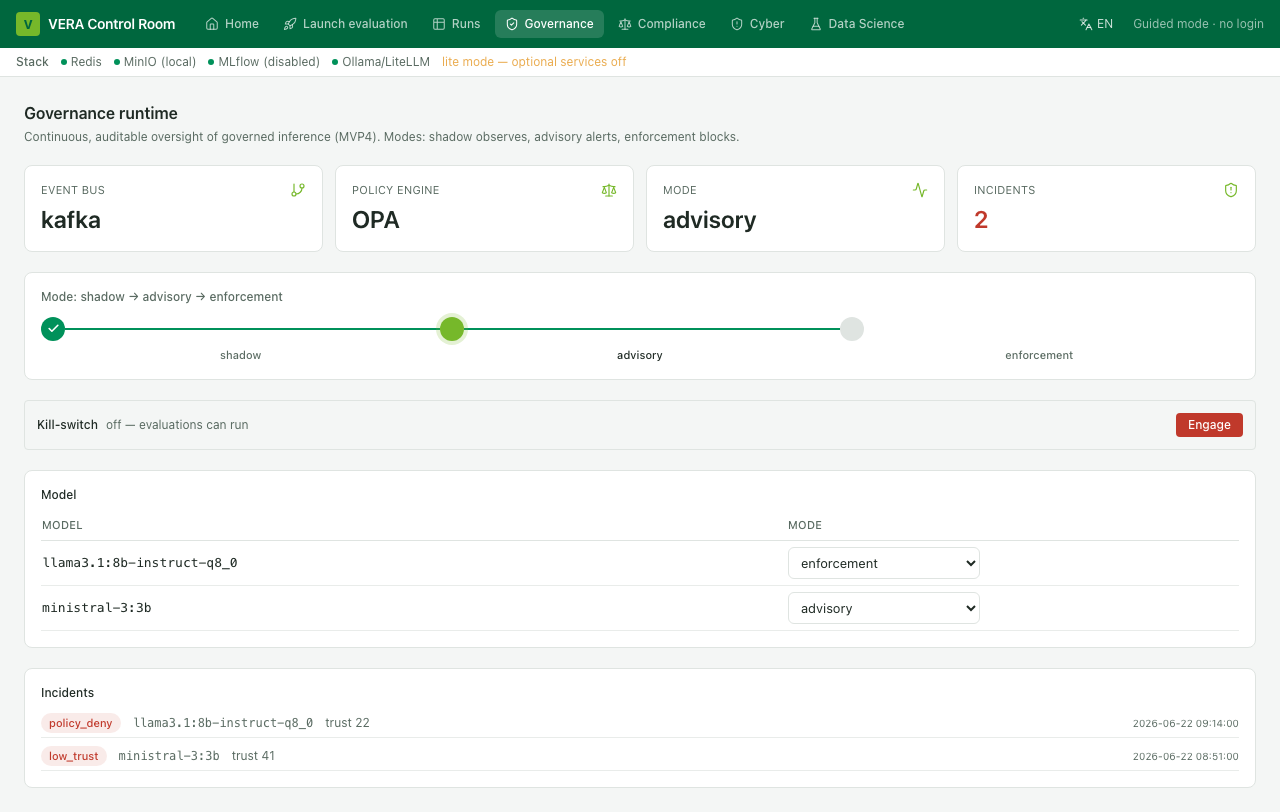
\includegraphics[width=\textwidth,height=0.42\textheight,keepaspectratio]{figures/shot_governance.png}
  \caption{Le panneau de gouvernance : modes par modèle (observation, consultatif, application), Trust Factor en direct, incidents et coupe-circuit.}
  \label{fig:app-gov}
\end{figure*}

\begin{figure*}[p]
  \centering
  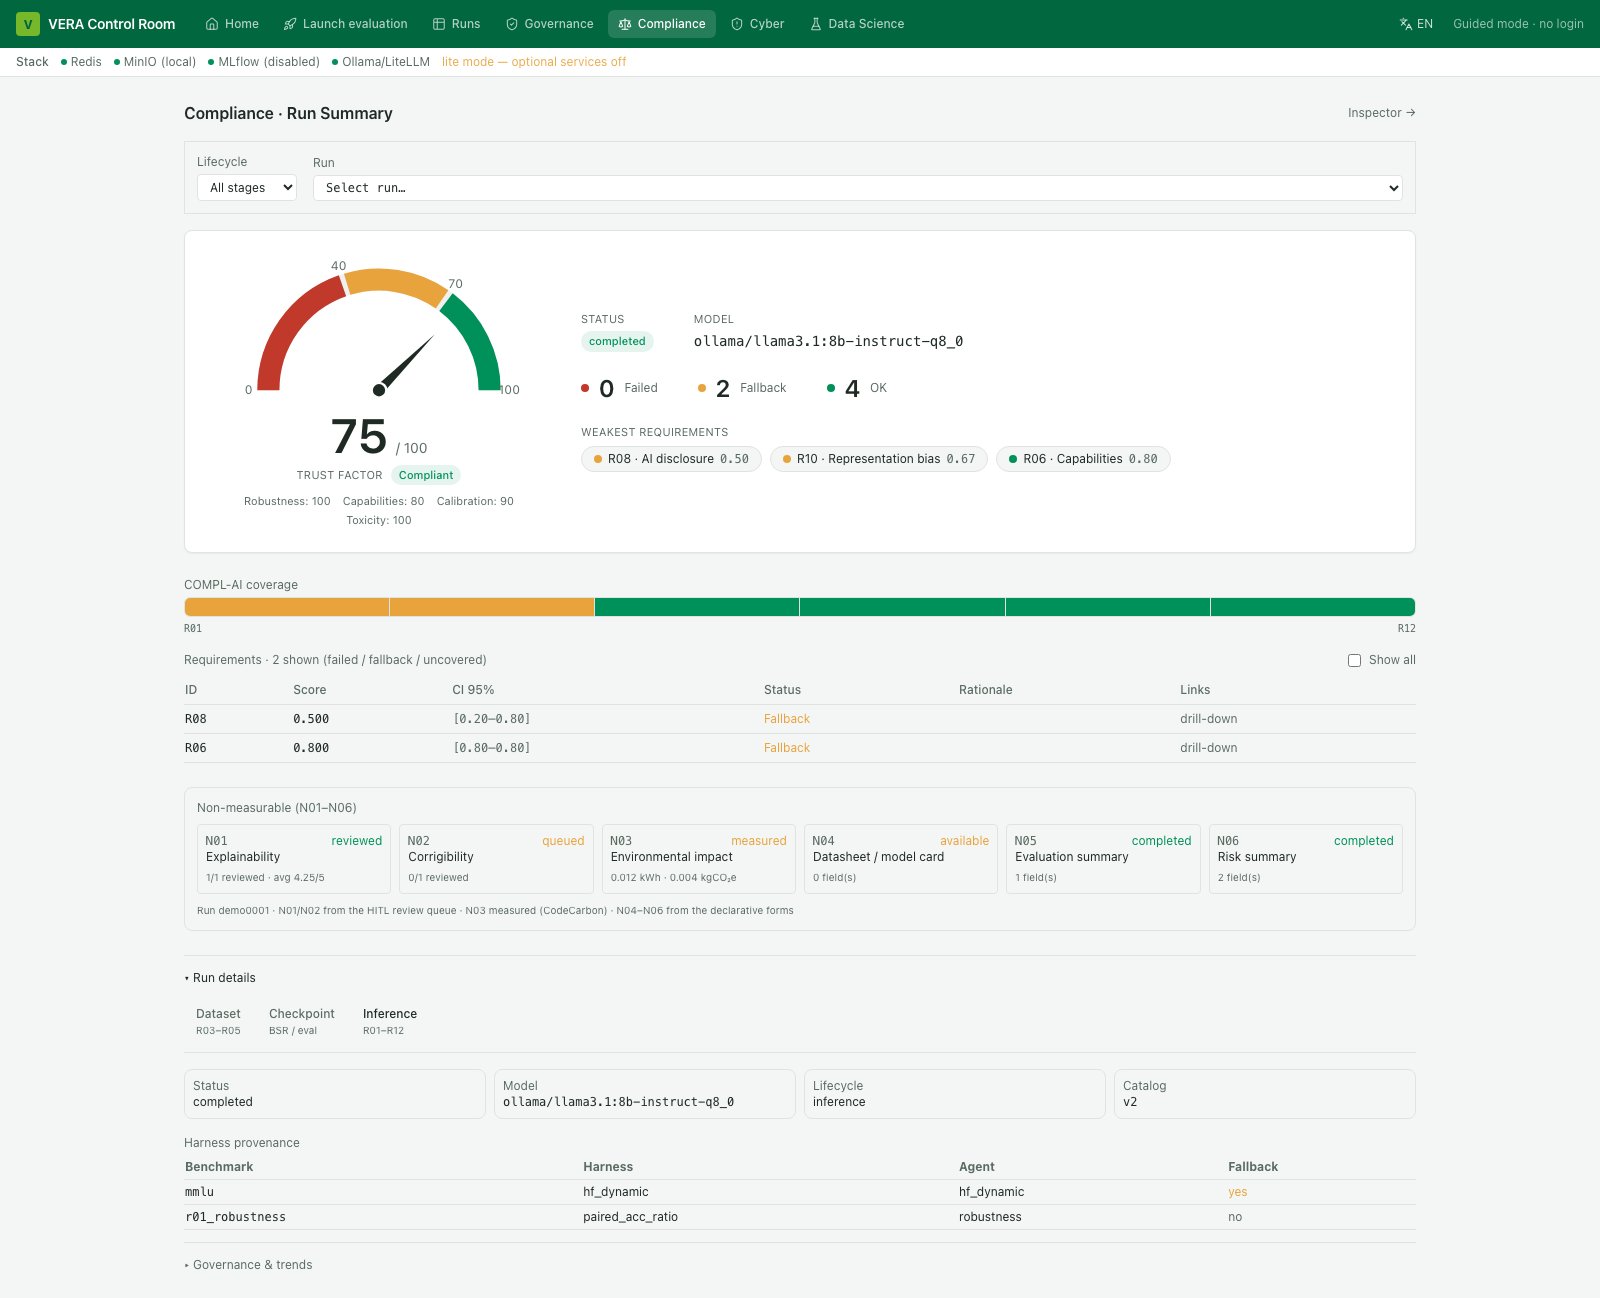
\includegraphics[width=\textwidth,height=0.42\textheight,keepaspectratio]{figures/shot_control_room_full.png}
  \caption{La vue complète d'une exécution avec les sections de détail dépliées : jauge d'accueil, bande de couverture, tableau de triage par statut, bandeau des exigences non mesurables (N01--N06), rail de cycle de vie, métadonnées d'exécution et provenance des exécuteurs.}
  \label{fig:app-full}
\end{figure*}

\end{document}
